\section{Fundamentals of Particle Image Velocimetry}

Particle Image Velocimetry, or PIV, is a class of methods employed in 
experimental fluid mechanics to measure instantaneous vector velocity fields by 
measuring the displacements of small visible particles (smoke or fog) which 
follow the motion of the fluid. Figure \ref{fig:quiver_example} shows a typical 
resulting vector field produced from measurements of a vortical flow. 
These two-dimensional vectors are defined from a thin sheet 
of illuminated fluid, captured in the planar volume. The velocity of the fluid 
is deduced by acquiring images of well entrained particles at precise times and 
measuring the displacement of those particles detected during the time 
interval. This is accomplished with the use of cameras for acquiring images 
and an intense laser light sheet to illuminate particles within the desired 
plane. This technique can be used to study flows in gases and liquids, and is 
derived from techniques originally developed to measure deformations on the 
surface of solid material \cite{arroyo1991,adrian1991}.

\vspace{20pt}
\begin{figure}[H]
	\centering
	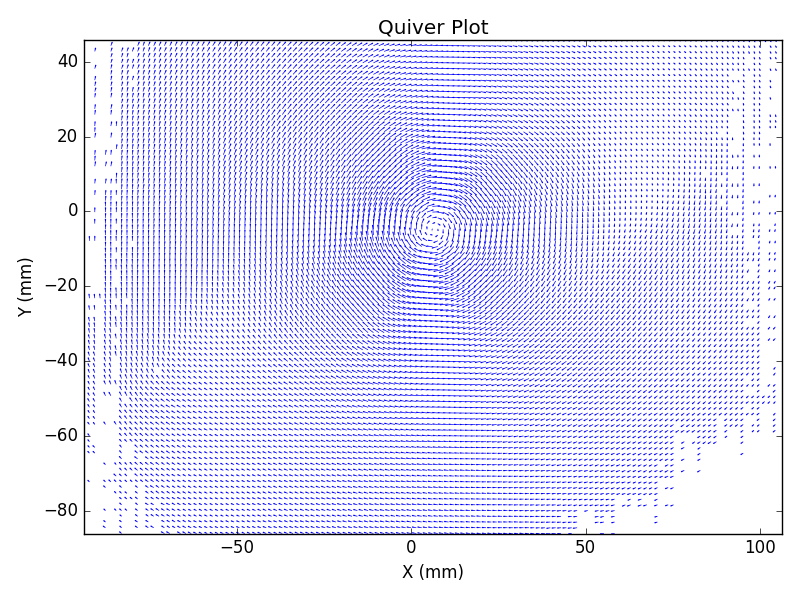
\includegraphics[width=5in]{figs/example_vortex_figs/example_quiver}
	\caption{Velocity vector field of a vortical flow structure as produced by 
	PIV.}
	\label{fig:quiver_example}
\end{figure}

 
\subsection{The Case for PIV}

Unlike other flow measurement techniques, PIV is considered to be a 
non-invasive method to directly measure particle displacements occurring during 
a precise time interval, and thus determine the particle velocity in the 
viewing plane. PIV is also capable 
of resolving vector measurements at many positions within a two-dimensional 
slice of the flow field simultaneously, while other measurement techniques 
require taking data at many locations sequentially over a much longer period 
of time. PIV measurements can also be used to infer lift and drag forces on a 
solid body \cite{noca1997}. Single camera PIV can measure the two components of 
the velocity vectors aligned with the image plane, but the PIV method is 
capable of resolving up to three dimensional velocities within an up to three 
dimensional volume of fluid flow with incremental increases 
in system complexity. The addition of a second camera can enable the 
measurement of the three-dimensional velocity vector, and a sweeping beam laser 
or holographic PIV architecture allows the interrogation of an entire volume of 
flow field instead of a "planar" slice 
\cite{barnhart1994,elsinga2006,kahler2000}.

Stereo PIV is widely used because it provides full velocity vector resolution, 
and requires only one additional camera and a slightly more complex 
calibration process and software to process the imagery. A stereo PIV system 
employing a  stationary sheet laser can resolve three dimensional mean velocity 
vectors and their associated fluctuations within a two dimensional slice of 
fluid flow. A 
two point correlation tensor containing important information about the 
turbulent structure of a flow can be obtained readily with PIV. The 
non-invasive nature of PIV, combined with the  ability to interrogate a flow 
volume very quickly for information with high dimensionality makes it 
exceptionally useful in fluid mechanics. \cite{adrian1991}

\subsection{PIV for the study of Turbulence}
The study of turbulent flows requires a large range of spatial and temporal 
velocity scales. Therefore, measurement techniques used to study turbulent 
phenomena require a significant spread between the lowest resolvable velocity, 
and the highest \cite{barnhart1994}. Although PIV has grown in popularity, it 
is not a complete replacement for more mature techniques including hot-wire 
anemometry. The most significant weaknesses of PIV are the relatively limited 
frequency response, and lower sampling rates than hot-wire anemometry.
It has been shown that the attenuation of the velocity and velocity derivative 
statistics is significantly higher with PIV than with hot-wire anemometry due 
to the volume averaging associated with PIV techniques, and the aerodynamic and 
inertial behavior of the particles in the flow.
However, correction procedures have been developed that have been shown to 
allow corrected PIV measurements of turbulent kinetic energy to agree closely 
with hot-wire anemometry measurements \cite{lavoie2007,kasagi1991}. 

Reynolds stresses can be extracted from the two point correlations averaged 
over 
an interrogation window. With this technique, one Reynolds stress value can be 
obtained for each of the smallest interrogation windows, which are typically 
several pixels in size. In this technique, the particle displacements are found 
by finding the peak of the correlation function of image pairs, transformed 
into velocities and divided into mean and fluctuating components typical 
of a Reynolds averaging approach. Alternatively, single-pixel resolution 
Reynolds stress measurements can be obtained by direct examination of the 
correlation function. This technique can estimate Reynolds stresses at an 
enhanced resolution with errors on the order of a few percent when employing a 
set of several thousand PIV image pairs \cite{scharnowski2011}.

\subsection{Principles of Planar PIV}

A simple planar PIV system consists of a double pulsed laser, light sheet 
forming optics, particle seed, a single lens camera, image digitization 
hardware, and a computer system for data storage and subsequent analysis. The 
optical geometry of a planar PIV experiment is shown schematically in Figure 
\ref{fig:mono_piv}.

\vspace{30pt}
\begin{figure}[H]
	\centering
	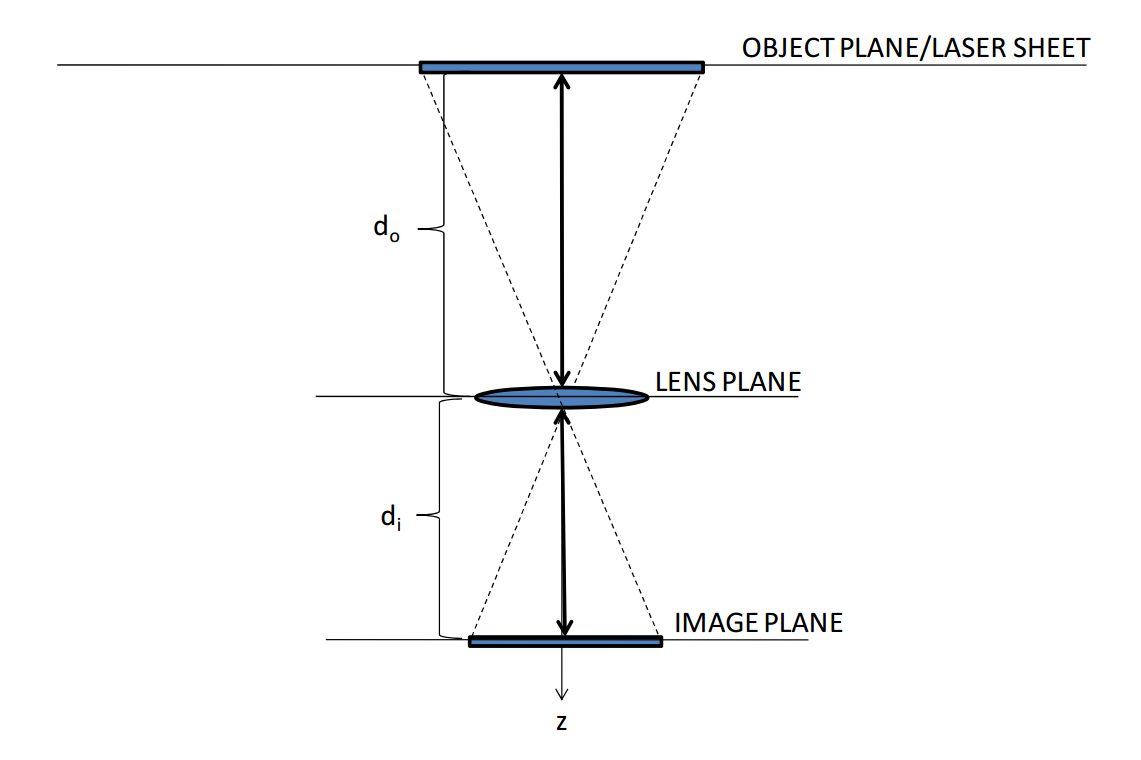
\includegraphics[width=5in]{figs/piv_method/mono_piv_optics}
	\caption{Single camera PIV system for mapping two dimensional velocity 
		vectors}
	\label{fig:mono_piv}
\end{figure} 

The 
underlying concept behind all PIV is that light scattered from the particles as 
they move through the illuminated flow field allows a pair of images to capture 
information about the motion of that particle. Double pulsed illumination is 
commonly employed in PIV systems, which allows two low cost lasers with the 
ability to pulse rather slowly to offset their pulses to achieve a 
satisfactorily small time interval ($dt$). The energy required to adequately 
illuminate a planar area of interest depends upon the size of that area, and 
the scattering properties of the particle seed. Solid state Nd:YAG lasers are 
typically used for this purpose \cite{adrian2011}. An $(X, Y, Z)$ coordinate 
system is defined within the light sheet that exists in a $(X, Y)$ 
space, and that can be related linearly to a 
coordinate system in the image plane of the camera in $(X_p, Y_p)$ pixel space. 
At a specific initiation time $t$, a laser light sheet is produced with a short 
duration pulse while the camera shutter is open to 
capture an image of the light scattering from particles within the flow domain. 
At some short time later, $t + dt$, a second light pulse occurs and a second 
image is taken. By measuring the pixel displacements $(\Delta X_p, \Delta 
Y_p)$ for a particle or group of particles in the image plane, and transforming 
the coordinates into the plane of the laser sheet, one obtains $(\Delta X, 
\Delta Y, \Delta Z)$. This coordinate transform can be obtained from precise 
information about the optical geometry of the system, or by direct measurement 
of calibration data \cite{fouras2007}.The method of direct measurement of a 
calibration target was employed in this research. 

The detection rate, accuracy, and reliability of PIV depends upon careful 
selection of experimental parameters. Kean and Adrian suggest a set of six 
important dimensionless quantities and ideal operating ranges that improve the 
chances of high quality PIV results \cite{keane1990}. The parameters 
are: (1) data validation criterion, (2) particle image density, (3) relative 
in-plane image displacement, (4) relative out-of-plane displacement, (5) 
velocity gradient, and (6) the ratio of the mean image diameter to the 
interrogation spot diameter \cite{keane1990,lawson1997b}. Steep flow velocity 
gradients create random errors, because the 
individual particle displacements cover a discreet range within an 
interrogation spot. Particle displacements should be restricted to 25\% of the 
interrogation spot diameter for in-plane velocities, and to no more than 25\% 
of the light 
sheet thickness in out-of-plane velocities. One way to mitigate both of these 
limitations is to use the highest resolution PIV possible, or by scaling the 
interrogation area down by altering the magnification on the camera lenses. 
Since the velocity profile of an axial vortex can contain high velocity 
gradients in the vicinity of the core, and both in-plane and out-of-plane 
velocities are expected to be high, the present experiments used 50mm lenses to 
allow each camera to focus on the smallest interrogation plane practical
\cite{prasad1992}.

\subsection{Principles of Stereo PIV}

Classical single camera PIV is only capable of capturing the projection of the 
velocity vector on the image plane. The out-of-plane component is lost 
completely, and the in-plane components are affected by unrecoverable error. In 
Stereo PIV, a pair of cameras may obliquely view the same plane and the entire 
three dimensional velocity vector can be inferred using the camera setup 
geometry. This technique 
includes tilting the backplanes of the cameras to satisfy the Scheimpflug image 
criteria and a dewarping function based on camera geometry to account for 
projective distortion \cite{willert1997}. An example of the geometric set up 
used by Willert to study the movement of a ring vortex through the 
interrogation plane is shown in Figure \ref{fig:stereo_piv}. Uncertainties 
associated with high out-of-plane motion in planar PIV are greatly reduced in 
stereo PIV \cite{lawson1997b,lawson1997}.

\vspace{32pt}
\begin{figure}[H]
	\centering
	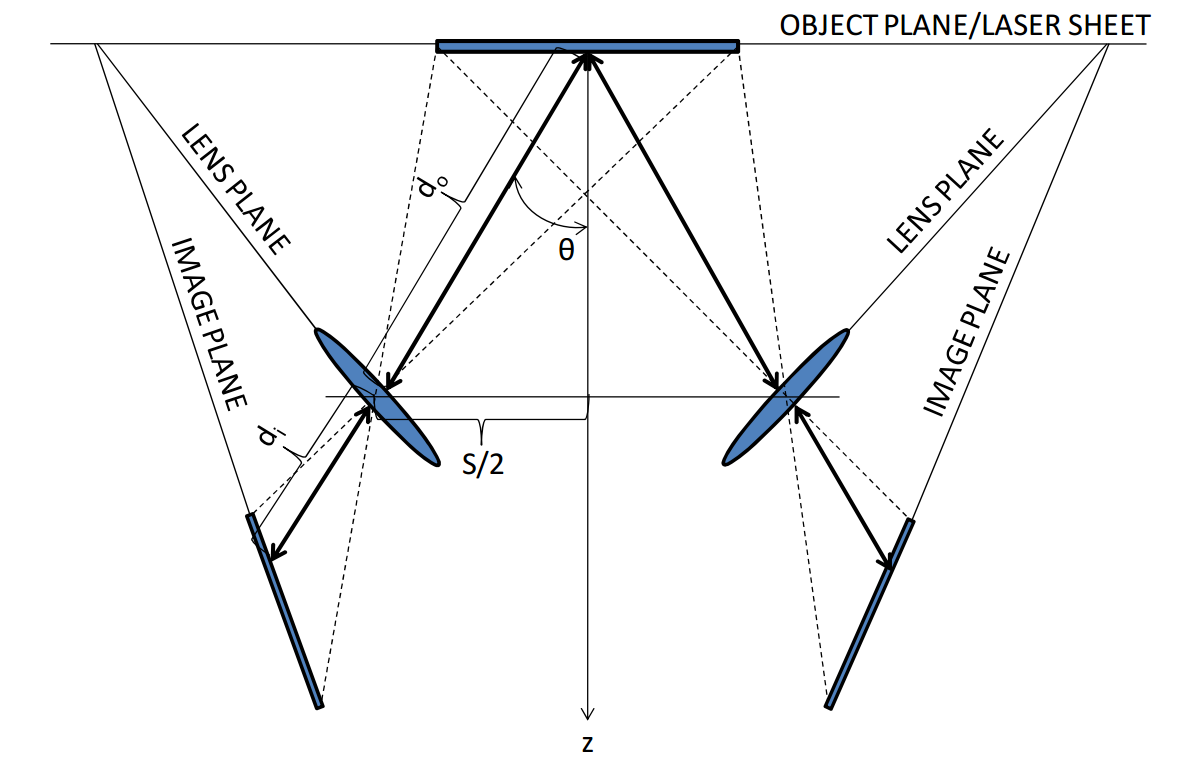
\includegraphics[width=5in]{figs/piv_method/stereo_piv_optics}
	\caption{Stereo camera PIV system for mapping three dimensional velocity 
		vectors}
	\label{fig:stereo_piv}
\end{figure}  
\vspace{16pt}

\subsection{Particles}

The ``Particles" part of the PIV acronym refers to the small, reflective solid 
or liquid spheres 
that are entrained within a flow and illuminated with 
an intense light source. It is assumed that 
the movement of the particles is representative of the fluid which propels them 
through the fluid, but this assumption deserves further examination 
\cite{roscoe1952}. Since particles have mass and inertia, the particle motion 
is a function of the viscous forces exerted upon them by the fluid, and by 
gravitational or magnetic body forces. As a particle is convected with the 
fluid and the local fluid encounters a change in direction, the particle cannot 
respond instantaneously. The exact response to rapid changes in velocity in the 
transporting fluid is of great interest to the study of turbulence. It has been 
found that lightweight 
particles have a tendency to collect in regions of high strain rate and low 
vorticity. However, extremely light particles exhibit weaker preferential 
concentration effects because they follow the fluid motion more closely, while 
relatively heavy particles become virtually insensitive to turbulent velocity 
fluctuations \cite{squires1990}. As the characteristic inertia and diameter of 
seed particles shrinks, they 
become capable of following 
smaller turbulent length scales, but the prime consideration for particles 
becomes the ability of a camera system to detect the light which scatters from 
them. The intensity of the light reflecting from a 
particles should be sufficient to reach 30\% to 50\% of the saturation level of 
the recording device. The controlling factors for intensity of reflected light 
are particle size, laser power, and refractive index \cite{adrian2011}. Thus, 
particles which are small enough to ensure sensitivity to turbulent structures 
on the time and length scales of interest must be small enough to respond to 
those turbulent fluctuation scales, but large enough to be detected. It has 
been demonstrated that particles with diameters on the order of 1 micrometer 
with a density much greater than the fluid can respond accurately to turbulent 
structures in air on the order of several thousand Hertz \cite{mei1996}.

The density of particle seeding must be sufficient for a correlation to be 
generated between frames for every small interrogation spot in the survey 
plane. In an instance where only one or two particles are visible in the first 
frame at the edge of an interrogation sector, then those particles exit the 
sector for the second frame, to be replaced by new particles 
entering the area from the other side, spurious results will be produced.


The present study used an industrial MDG MAX 
3000APS fog machine to produce mineral oil particles to use as seed. These 
particles are between 0.5 and 0.7 microns in size with a material density of 
838 $kg/m^3$. The scales at which an entrained particle can 
be assumed to represent the velocity of the flow with less than 1\% error is 
well described by stokes number, which expresses the relative importance of 
particle inertia to viscous drag on the particle trajectory:

\begin{equation}
St = \frac{\rho_p d^{2}_{p}}{18 \mu} \frac{\Delta u}{\delta}
	\label{eq:stokes}
\end{equation}

\noindent
where $\rho_p$ is the density of the particle, $d_p$ is the diameter, $\mu$ is 
the fluid viscosity, $\Delta u$ is the characteristic velocity change, and 
$\delta$ is the characteristic length scale. Stokes numbers less than 0.1 
produce particle tracing errors at the 1\% level and below \cite{brennen2005}.
Equation \ref{eq:stokes} can be rearranged to solve for the smallest length 
scales that can be represented by 0.6 micron mineral oil droplets with a 
density of 838 $kg/m^3$ suspended in air. Using a conservative estimate of a $1 
m/s$ characteristic $\Delta u$, This exercise reveals that the length over 
which particles can accurately respond to a $1 m/s$ characteristic velocity 
change is of the order of 0.01 $mm$. It is important to note that demonstrates 
the particles ability to respond very well to \textit{unsteady} forcing by 
fluctuating fluid velocities. It is perhaps intuitive that for a strong 
sustained rotational motion (much like a rigid body) such as a vortex core, any 
particles with density 
greater than the fluid will eventually be thrown out of the core, as 
demonstrated by \cite{lang1999}, and visible in Figure 
\ref{fig:vortex_core_particles}. This outward motion of the seed particles that 
is not representative of fluid motion creates a small outward bias in radial 
velocity measurements, particularly within the core boundary.

\vspace{32pt}
\begin{figure}[H]
	\centering
	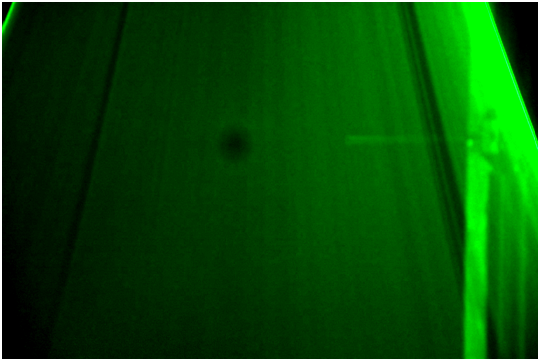
\includegraphics[width=4in]{figs/piv_method/vortex_core}
	\caption{Contrast enhanced image of an illuminated cross section showing a 
		low particle density in the vortex core.}
	\label{fig:vortex_core_particles}
\end{figure}
\vspace{16pt}

\subsection{Image processing}

There are multiple methods for extracting vector fields from images of 
particles. A commonality between all methods is the use of a correlation 
function to distinguish actual particle displacements from two or more 
sequential images. The correlation map is 
computed by taking the inverse fast Fourier transform (FFT) of the product of 
the FFT of the first image, and the complex conjugate of the FFT of the second 
image, then adjusting for up-sampling by dividing by the original up-sampling 
factor. Displacement is measured by finding the peak of correlation map 
between a small sector of each image, where $C_{map}$ is given by

\begin{equation}
C_{map} = FFT^{-1} * [F_A \times conj(F_B) ]
\label{eq:correlation_map}
\end{equation}

\noindent
and $F_A$ is the fast Fourier transform of 
image $A$, at time $t=0$ and $F_B$ is the fast Fourier transform of image $B$ 
at time $t=dt$. This process is repeated many times to create a vector field of 
pixel displacements. In the simplest case, these correlation maps are 
considered individually, and the absolute highest peak is used to determine the 
mean pixel displacement within a sector. The Hart method, employed in the 
present study, improves upon this general approach by utilizing an element by 
element comparison of correlation tables from adjacent sectors to remove false 
peaks \cite{hart1998,hart1999}.

The mathematics behind derivation of velocity vector fields from stereo image 
pairs is based upon coordinate transformations from pixel coordinates to real 
coordinates. That is, 

\begin{equation}
x_L= X\frac{dx_L}{dX} + Y\frac{dx_L}{dY} + Z\frac{dx_L}{dZ}
\label{eq:piv_to_real1}
\end{equation}

\begin{equation}
x_R= X\frac{dx_R}{dX} + Y\frac{dx_R}{dY} + Z\frac{dx_R}{dZ}
\label{eq:piv_to_real2}
\end{equation}

\begin{equation}
y_L= X\frac{dy_L}{dX} + Y\frac{dy_L}{dY} + Z\frac{dy_L}{dZ}
\label{eq:piv_to_real3}
\end{equation}

\begin{equation}
y_R= X\frac{dy_R}{dX} + Y\frac{dy_R}{dY} + Z\frac{dy_R}{dZ}
\label{eq:piv_to_real4}
\end{equation}

\noindent
where $x_L$, $x_R$, $y_L$ and $y_R$ are the pixel locations in the x 
direction on the left and right cameras; similarly for the y direction on the 
left and 
right cameras respectively. Symbols $X$, $Y$, and $Z$ are real spatial particle 
displacements in the interrogation plane. The set of twelve derivatives are 
pixel displacement sensitivity coefficients, which are determined by employing 
a calibration process which involves taking pictures of a matrix of bright 
dots arranged on a physical calibration target with a known separation distance 
between 
each dot. Once all twelve calibration coefficients are determined, the set of 
equations is actually over constrained, since there are four equations and only 
three unknowns, justifying a least squares best fit to map measurements from 
the image plane to the real plane. In the case of this study, 
INSIGHT\textsuperscript{\textcopyright}  software was used to generate this 
set of calibration 
coefficients 
\cite{fouras2007}.

The image is 
up-sampled to higher resolution to allow sub-pixel displacements to be 
measured, thus preventing accuracy limitations associated with the physical 
dimensions of each pixel. The image is divided typically into grids 16 by 16 
pixels in size, with 50\% overlap with surrounding grids to ensure particles 
which started inside the sector at $t=0$, but begin to exit the sector at 
$t=dt$, are still identifiable.  


Figure \ref{fig:piv_sector_0up} shows a sample of two side by side images taken 
several microseconds, ($dt$) apart without any up-sampling. Figure 
\ref{fig:piv_sector_overlay_fft_0up} shows a sample of the same two images 
layered on top of each other to show the apparent horizontal displacement 
between the two images. The two dimensional correlation map shows a clear peak 
down at four pixels in the $X$ direction and zero pixels in the $Y$ direction.

\vspace{32pt}
\begin{figure}[H]
	\begin{subfigure}{.49\textwidth}
		\centering
		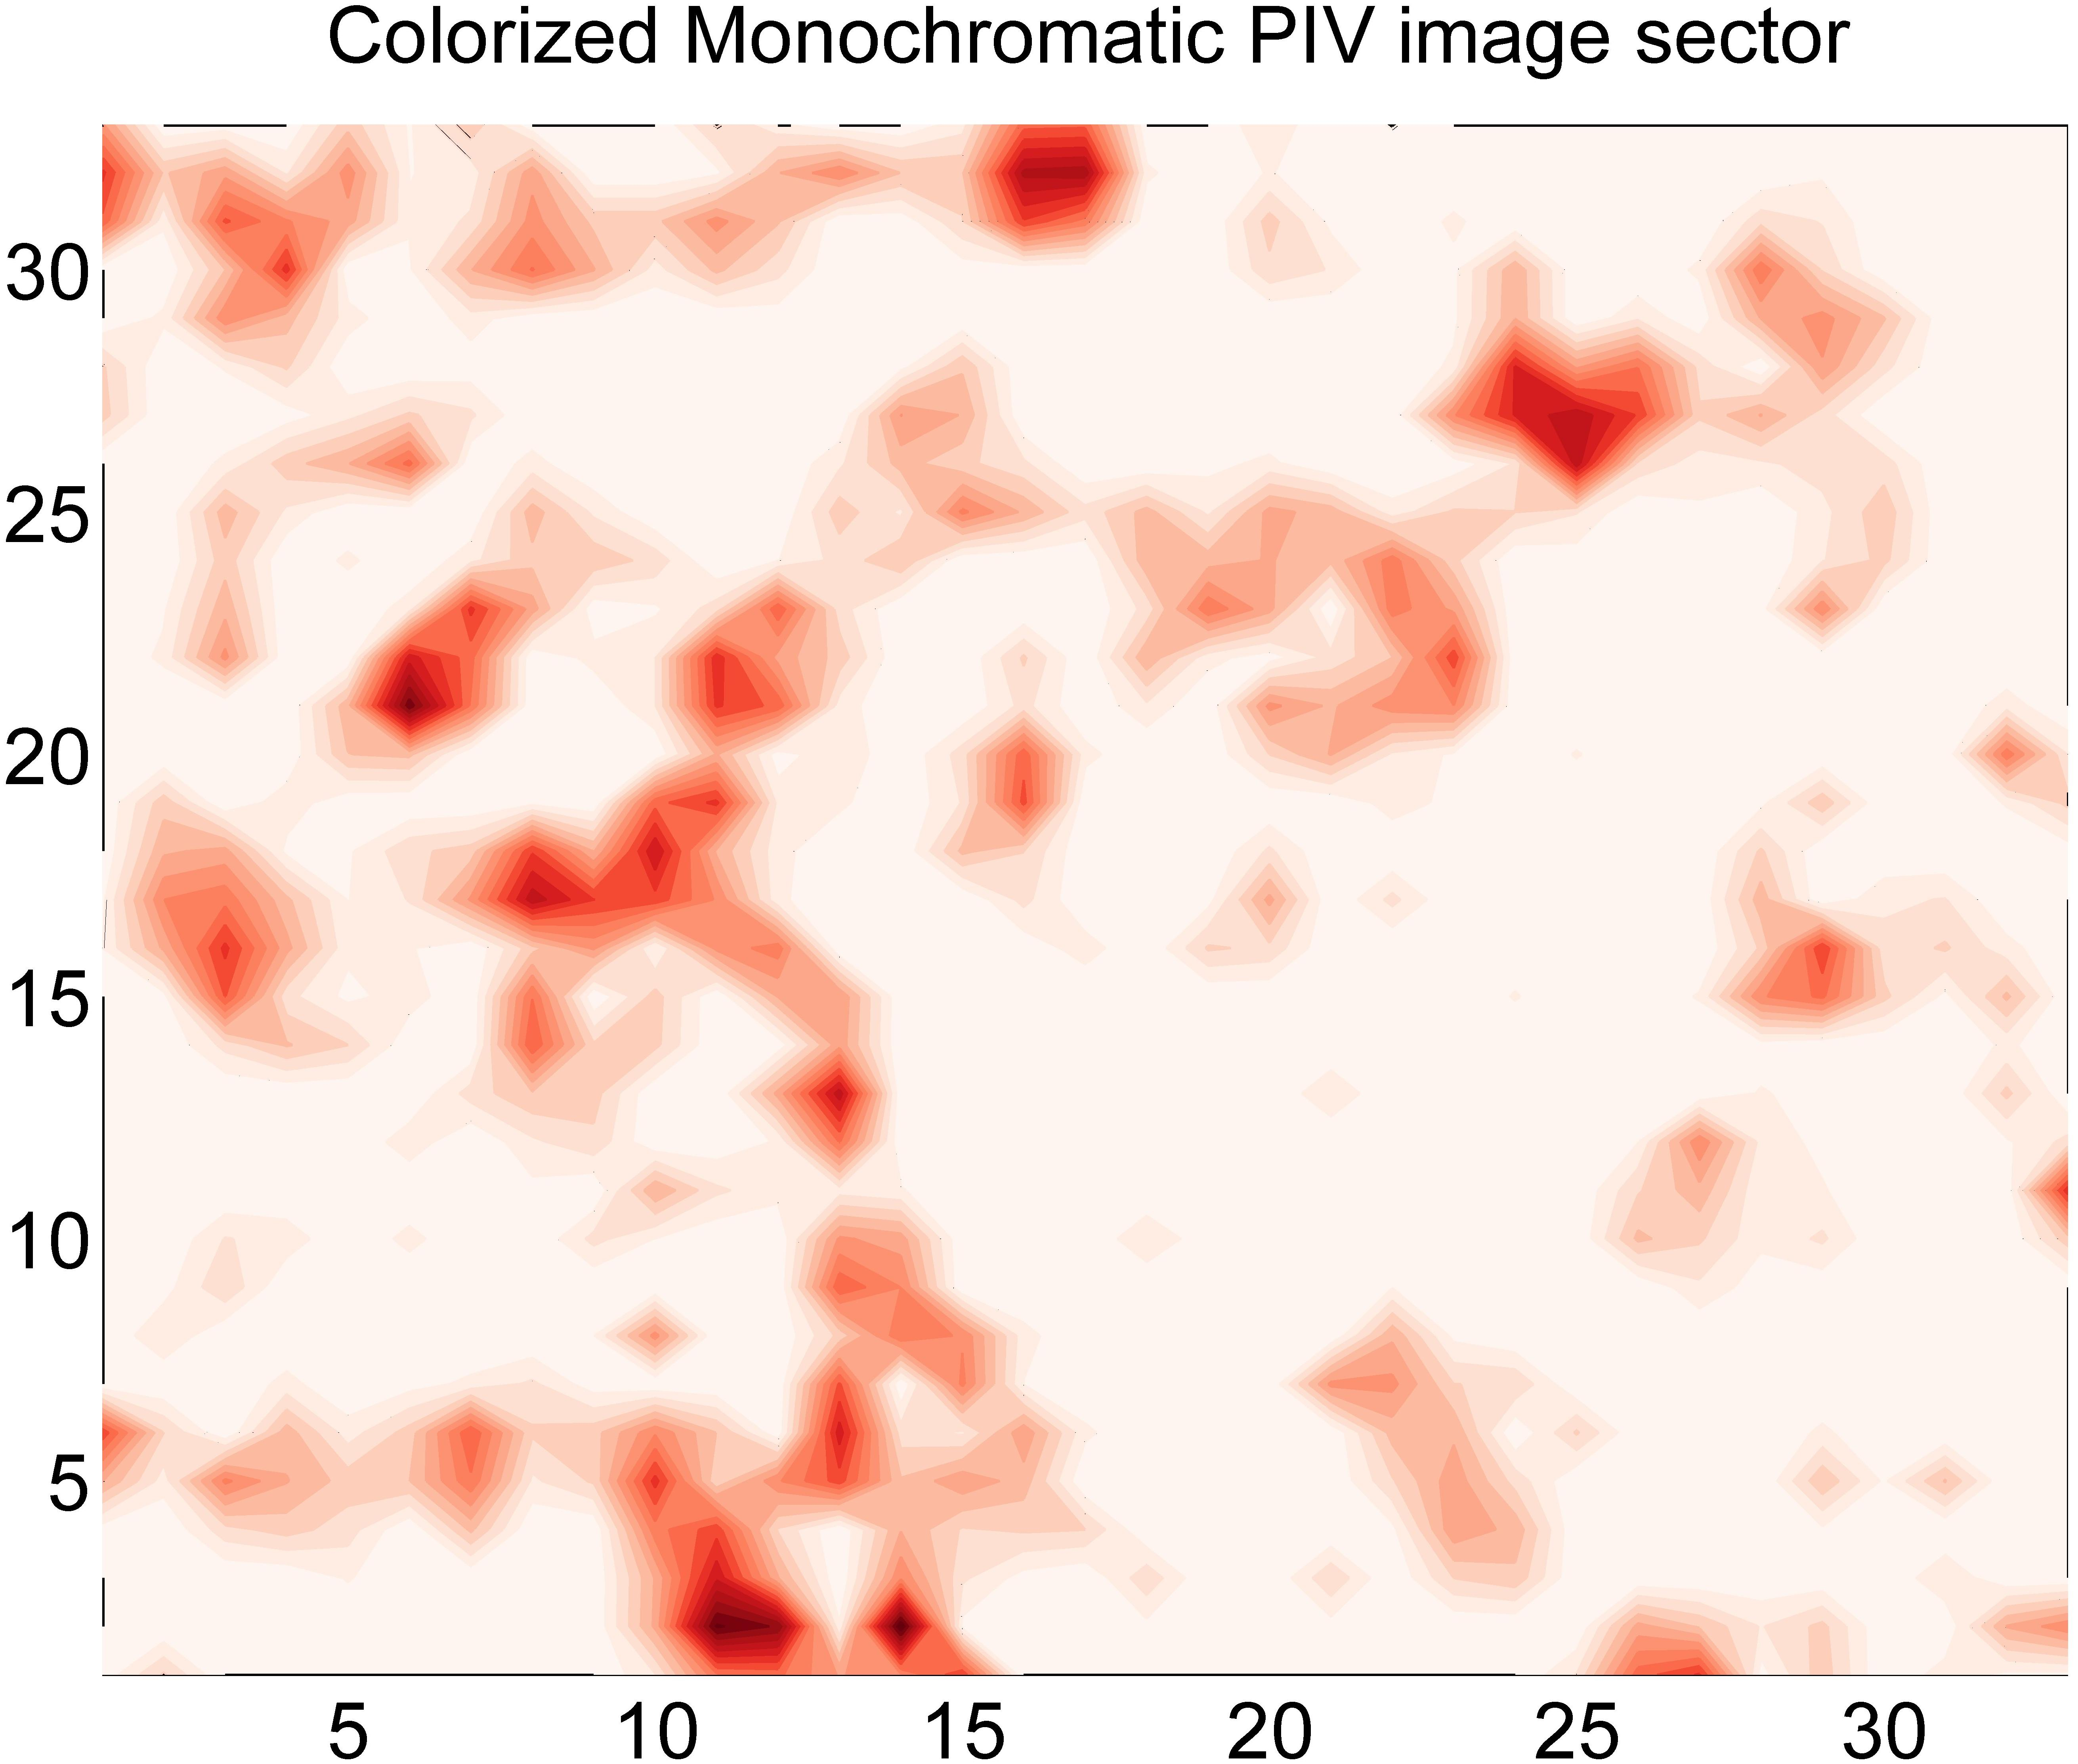
\includegraphics[width=.9\linewidth]{figs/piv_method/pive_figa_order0}
	\end{subfigure} 
	\begin{subfigure}{.49\textwidth}
		\centering
		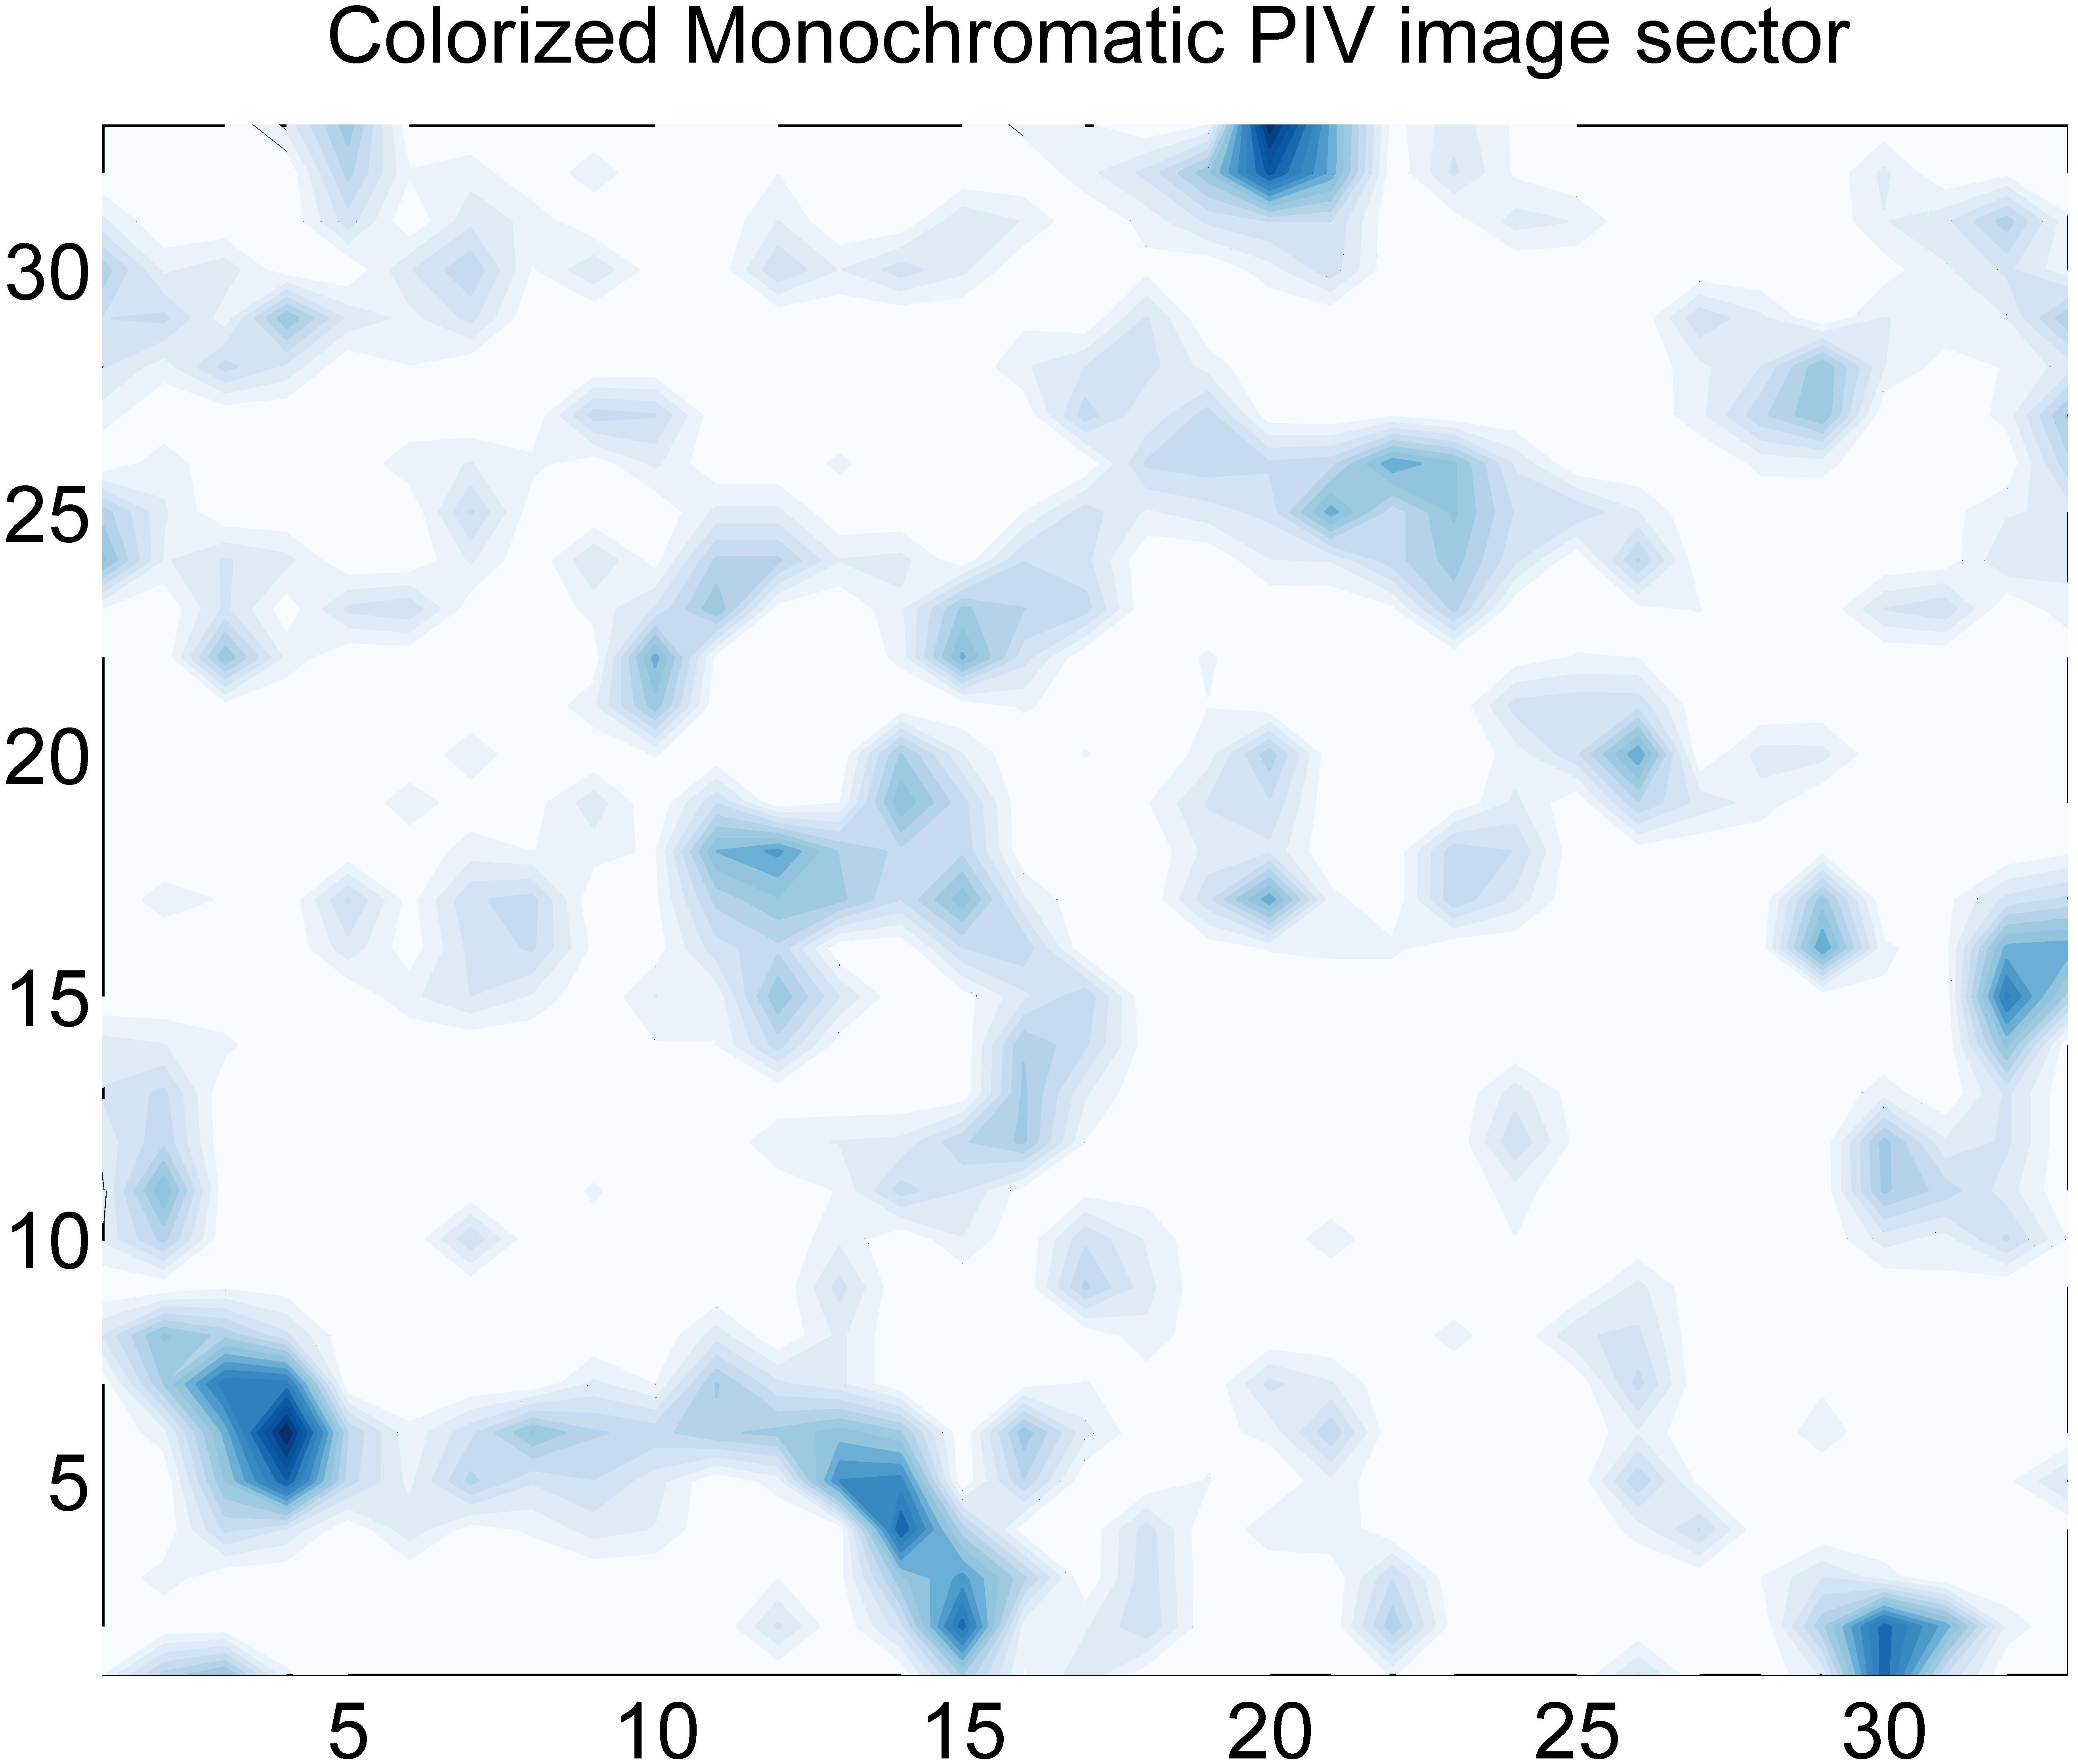
\includegraphics[width=.9\linewidth]{figs/piv_method/pive_figb_order0}
	\end{subfigure}	
	\caption{Colorized 32x32 pixel contour images at $t=0$ (left), and $t=dt$ 
		(right), no up sampling.}
	\label{fig:piv_sector_0up}
\end{figure}
\begin{figure}[H]
	\begin{subfigure}{.49\textwidth}
		\centering
		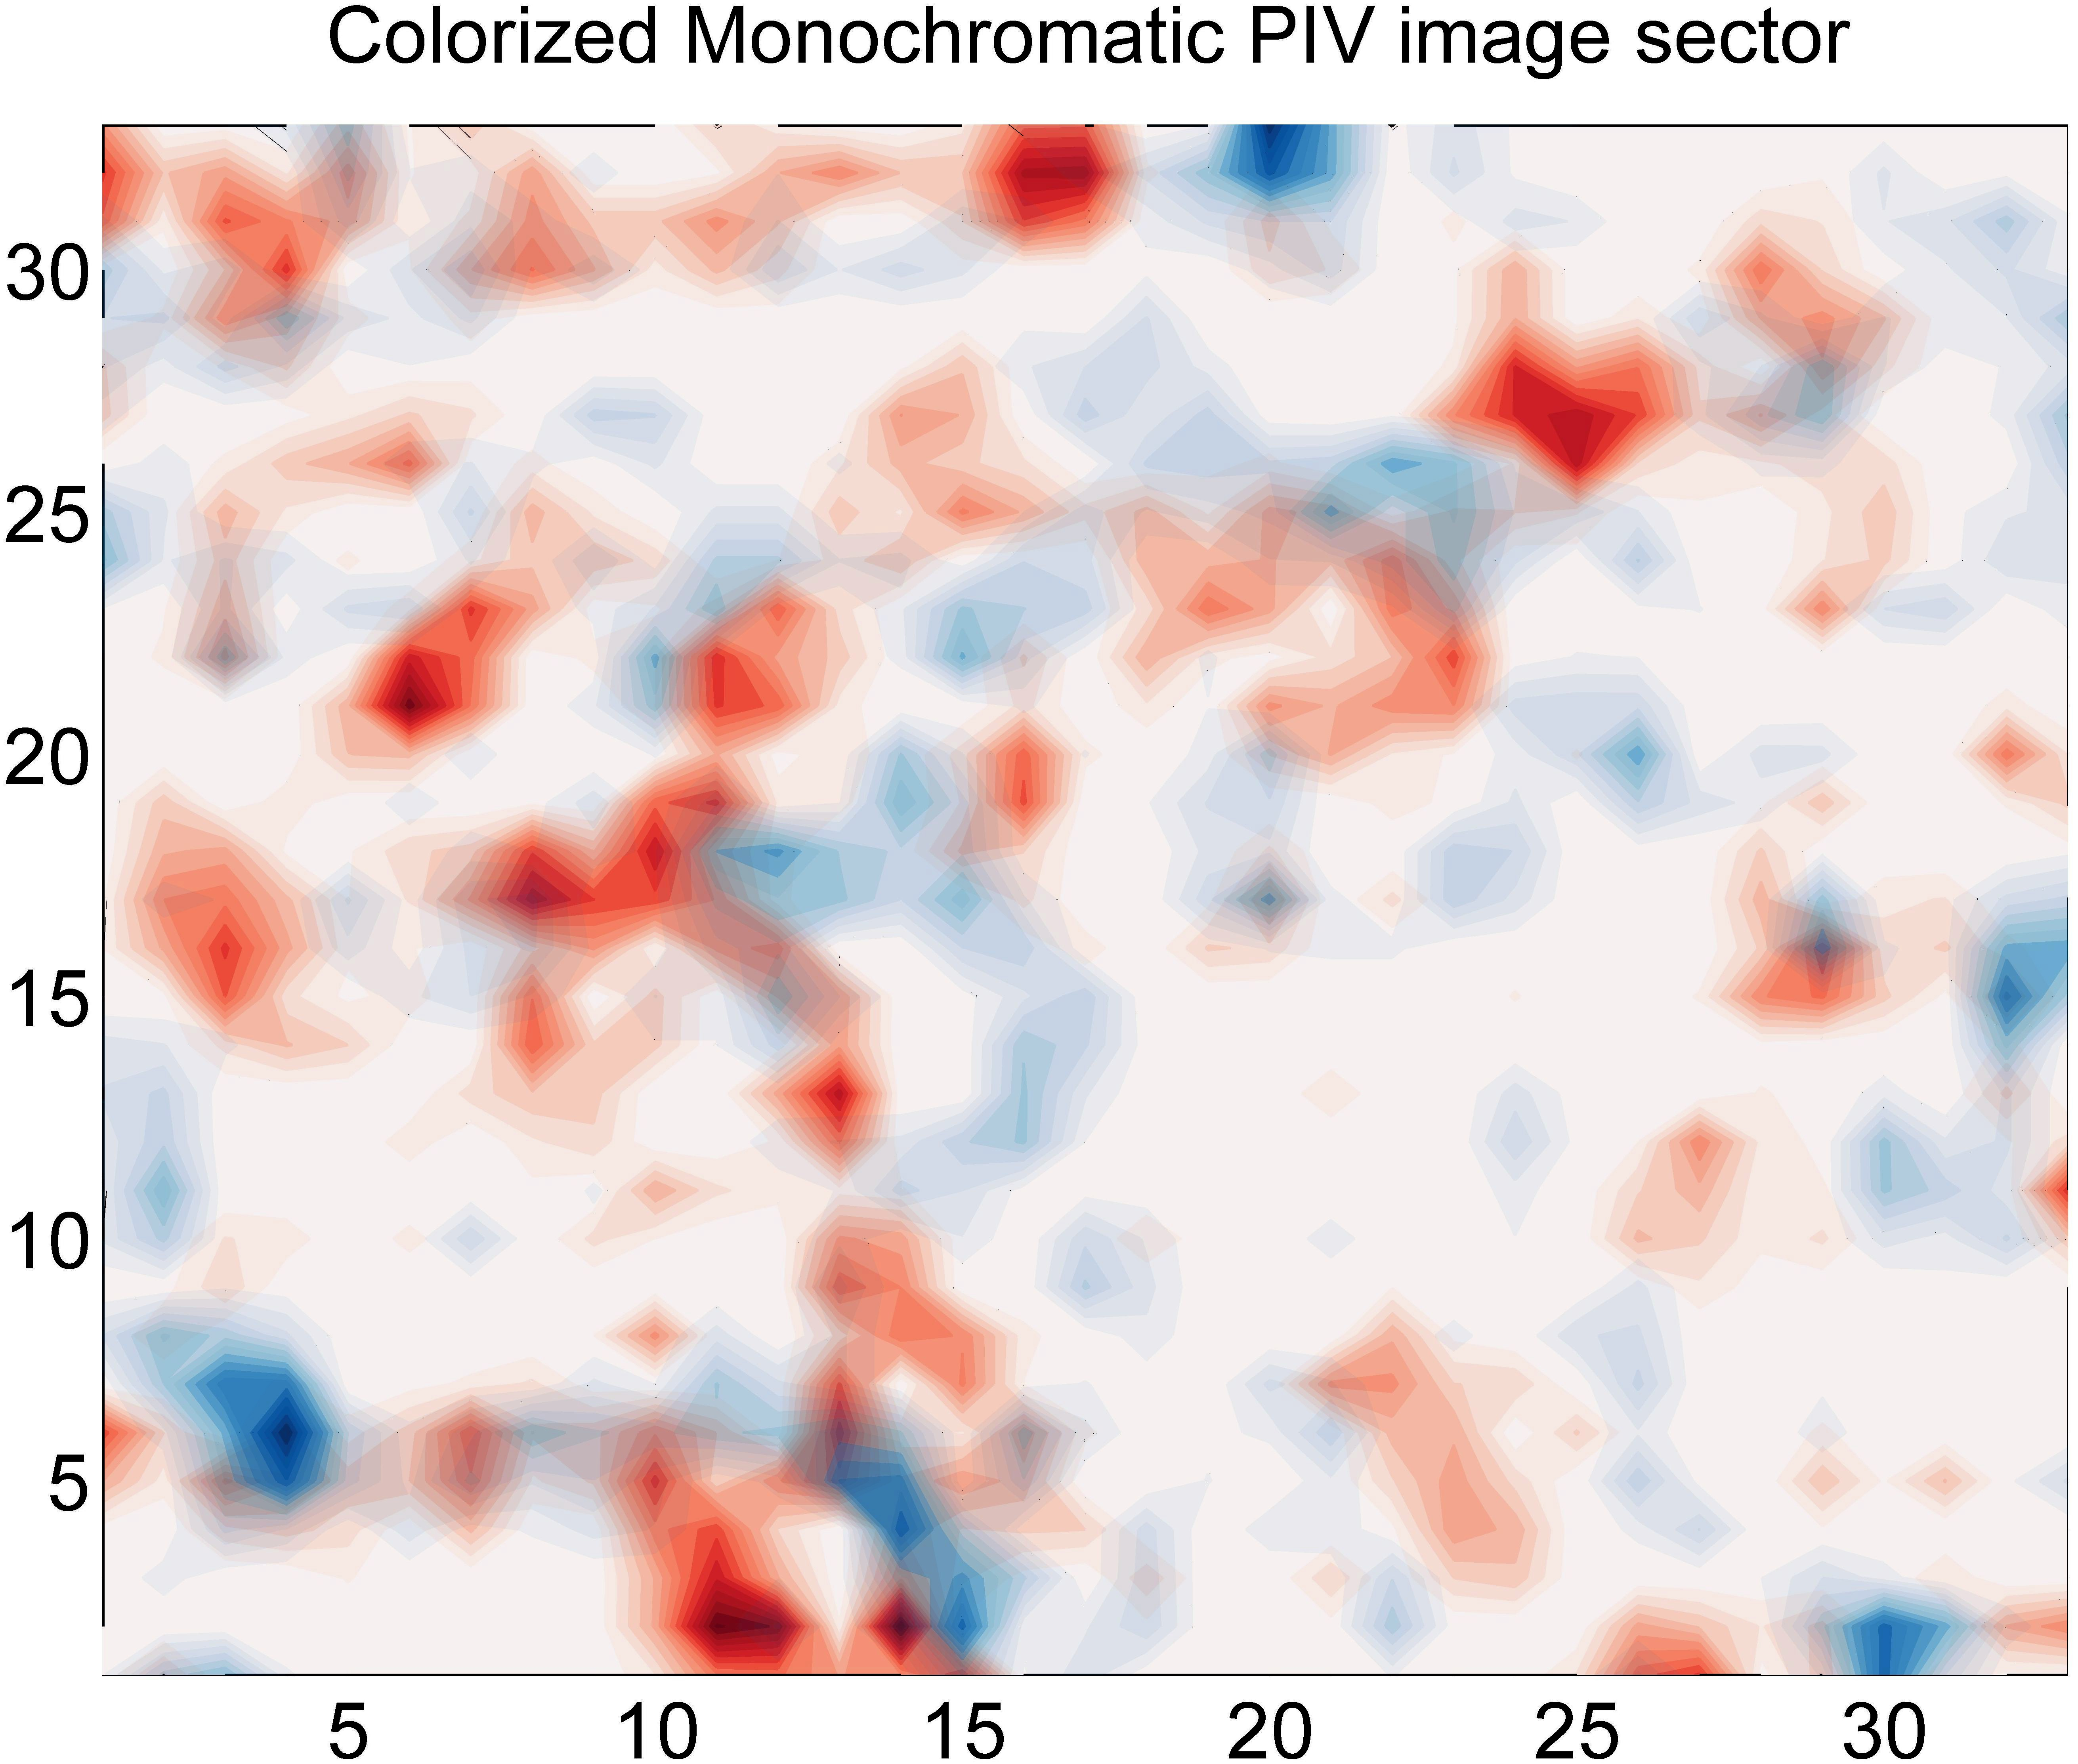
\includegraphics[width=.9\linewidth]{figs/piv_method/pive-fig_order0}
	\end{subfigure} 
	\begin{subfigure}{.49\textwidth}
		\centering
		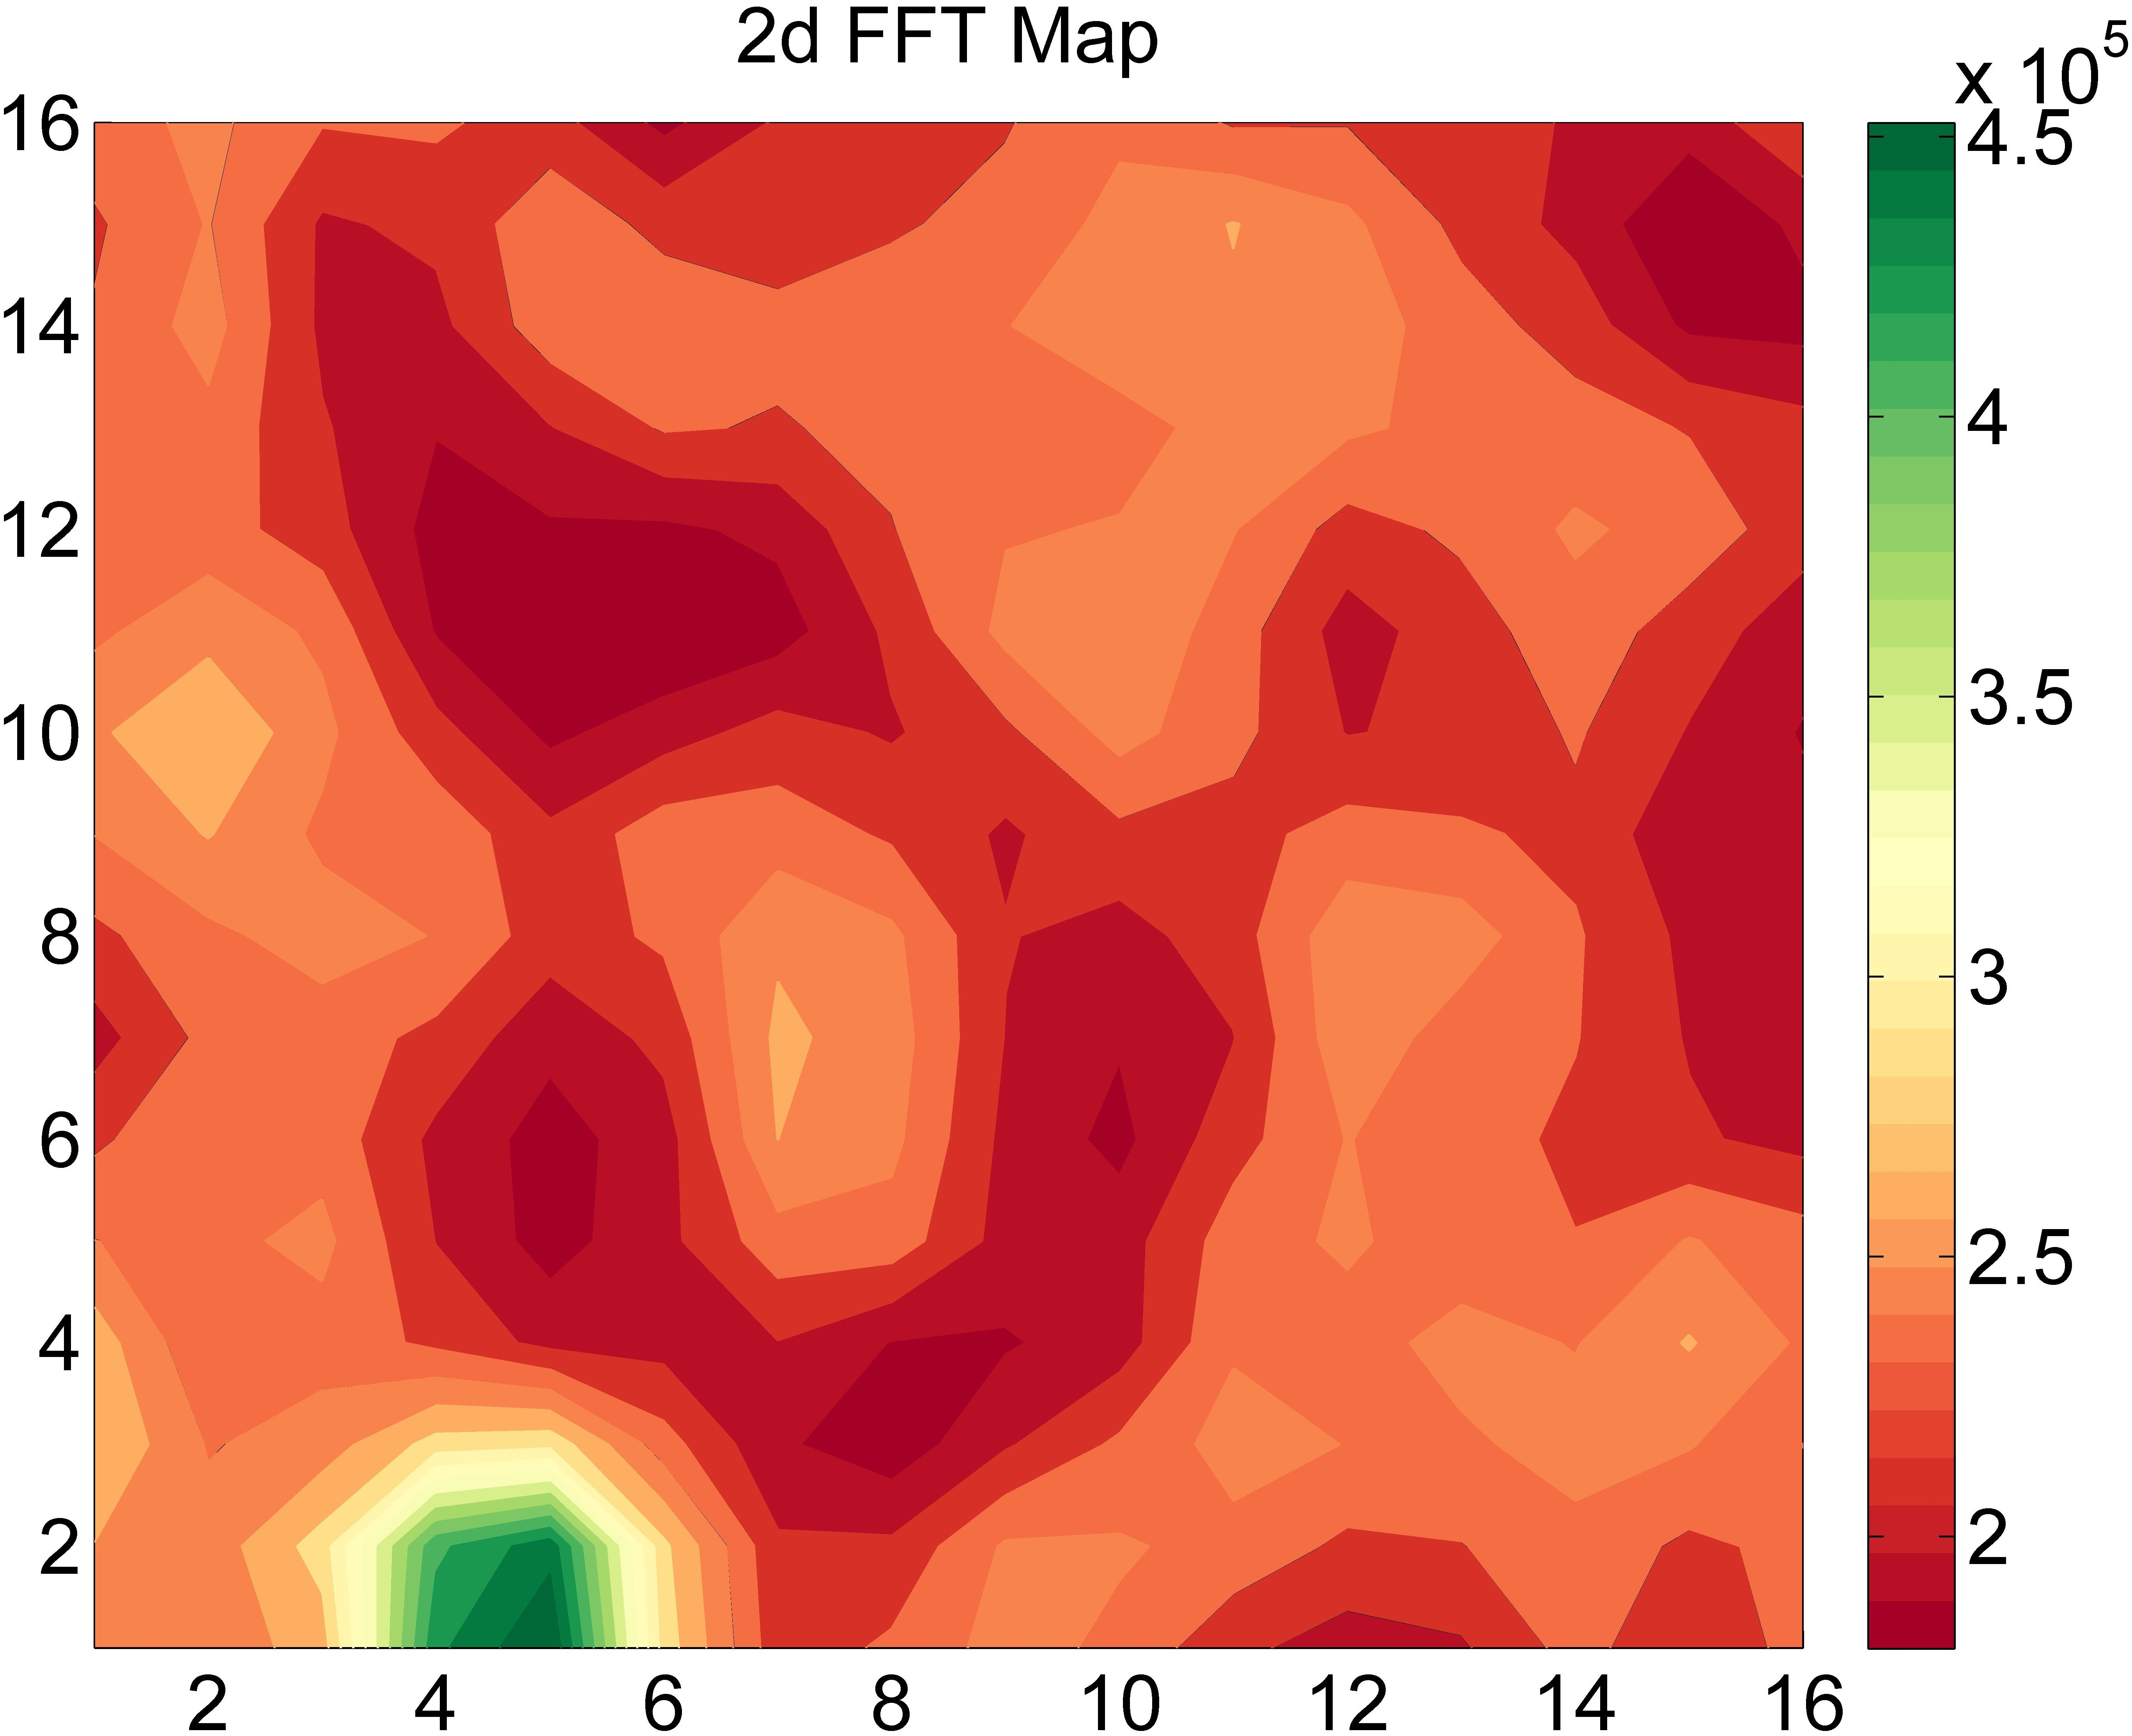
\includegraphics[width=.9\linewidth]{figs/piv_method/pive_fft_order0}
	\end{subfigure}	
	\caption{Overlaid sector snapshots (left) and corresponding correlation 
		map (right), no up sampling.}
	\label{fig:piv_sector_overlay_fft_0up}
\end{figure}
\vspace{32pt}

Every up sampling doubles the dimensions of the sector, quadrupling the number 
of pixels and increasing the sub-pixel resolution by a factor of two. The same 
set of figures is repeated for the same image with 6th order bilinear up 
sampling in Figures \ref{fig:piv_sector_6up} and
\ref{fig:piv_sector_overlay_fft_6up}. Note that the images are much smoother, 
and the images have been sampled sufficiently to make a very finely spaced grid.
It is important to note that while bilinear up sampling is used for this
example, any other two dimensional method such as cubic may be used.

\vspace{32pt}
\begin{figure}[H]
	\begin{subfigure}{.49\textwidth}
		\centering
		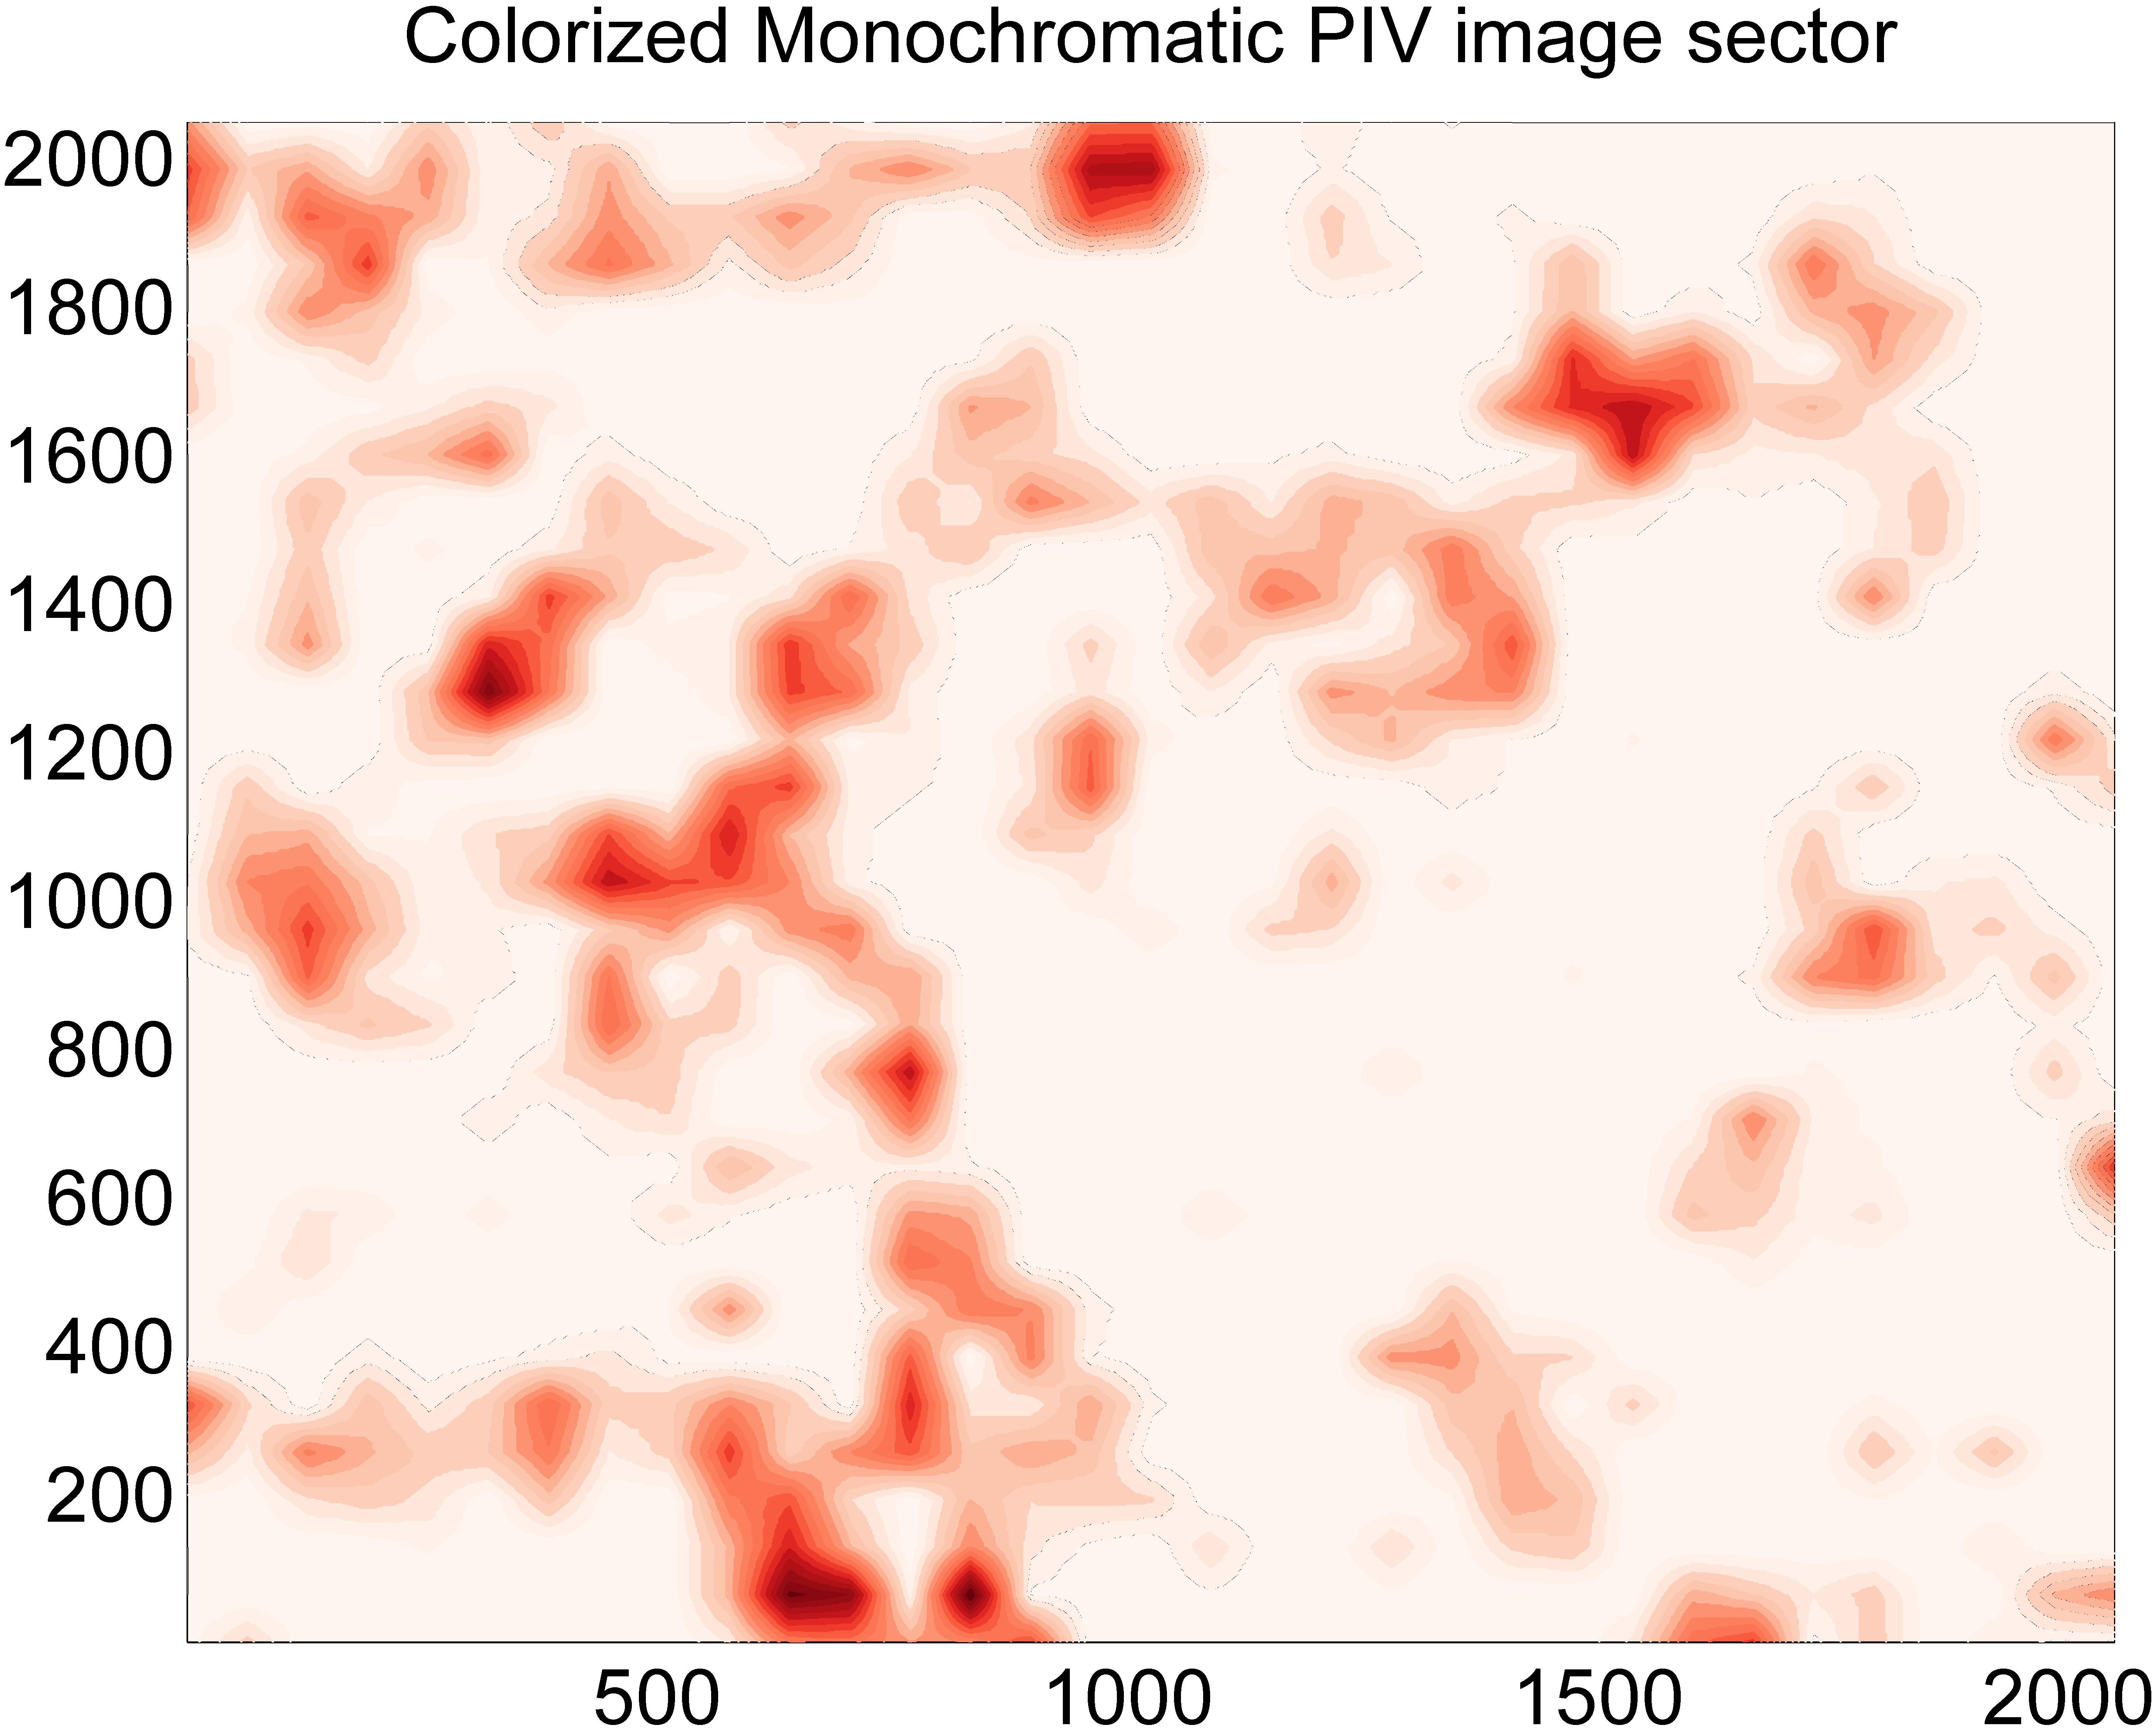
\includegraphics[width=.9\linewidth]{figs/piv_method/pive_figa_order6}
	\end{subfigure} 
	\begin{subfigure}{.49\textwidth}
		\centering
		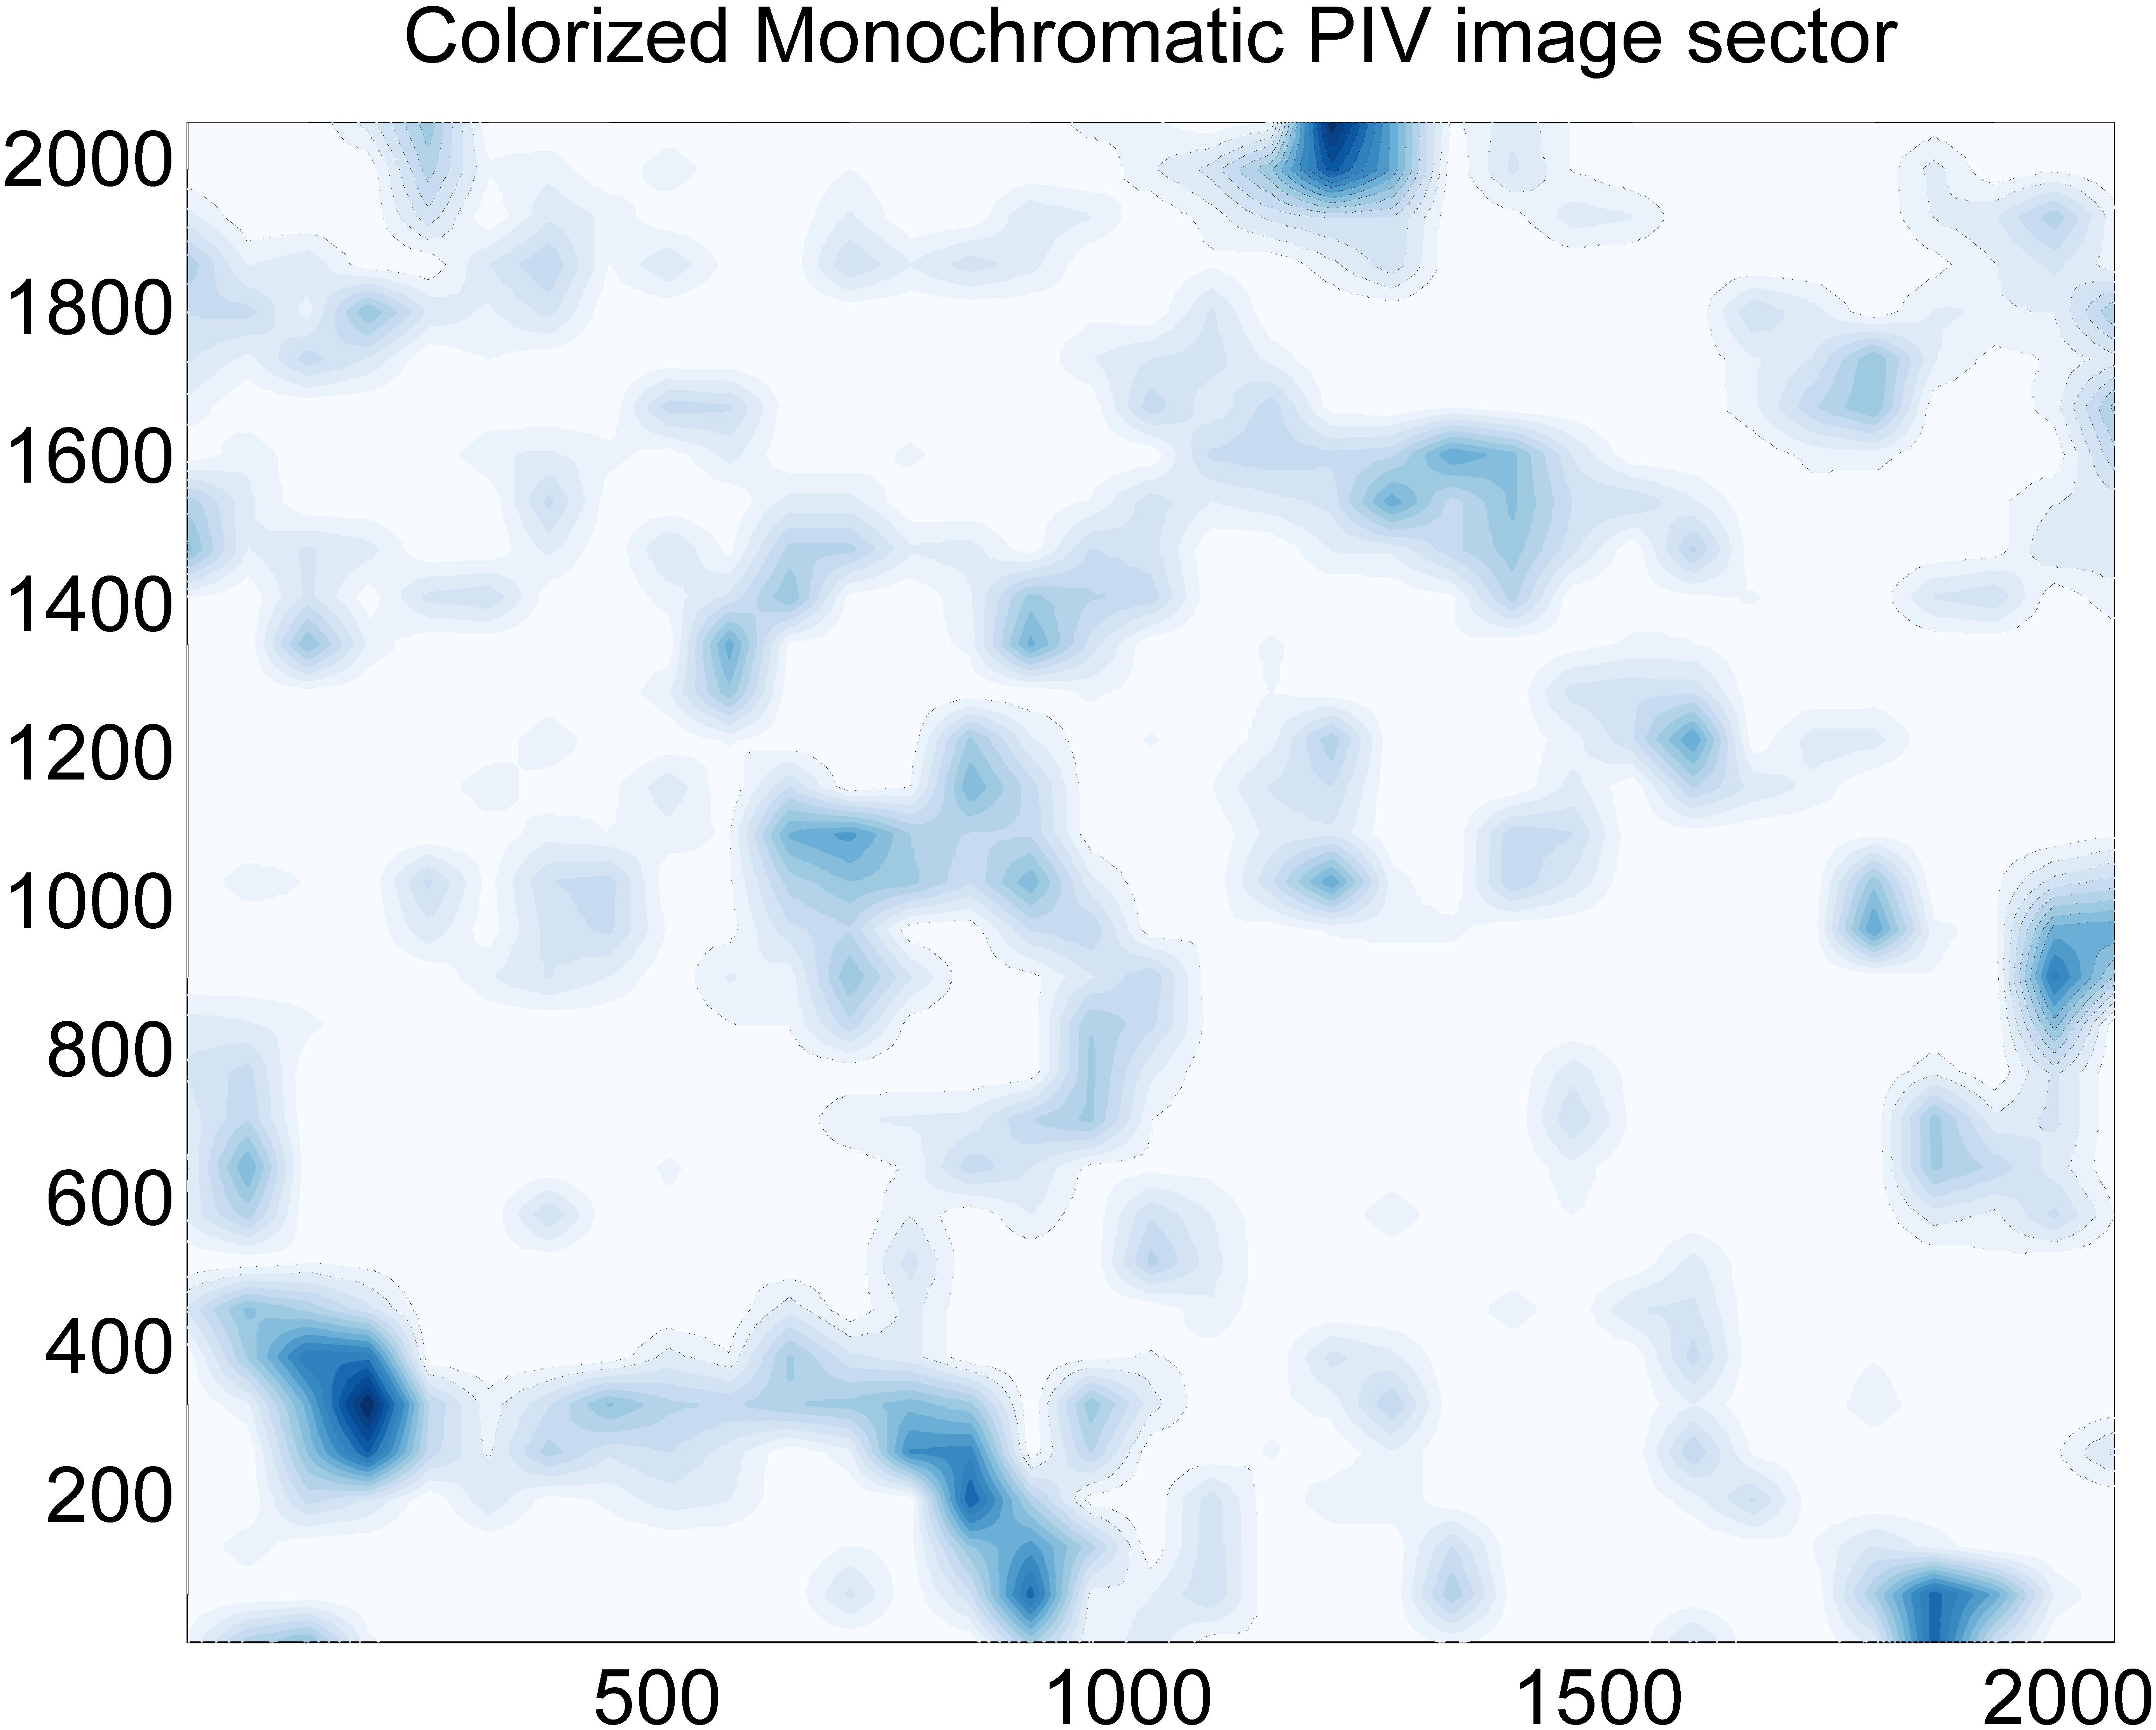
\includegraphics[width=.9\linewidth]{figs/piv_method/pive_figb_order6}
	\end{subfigure}	
	\caption{Colorized 32x32 pixel contour images at $t=0$ (left), and $t=dt$ 
		(right), 6th order up sampling.}
	\label{fig:piv_sector_6up}
\end{figure}
\begin{figure}[H]
	\begin{subfigure}{.49\textwidth}
		\centering
		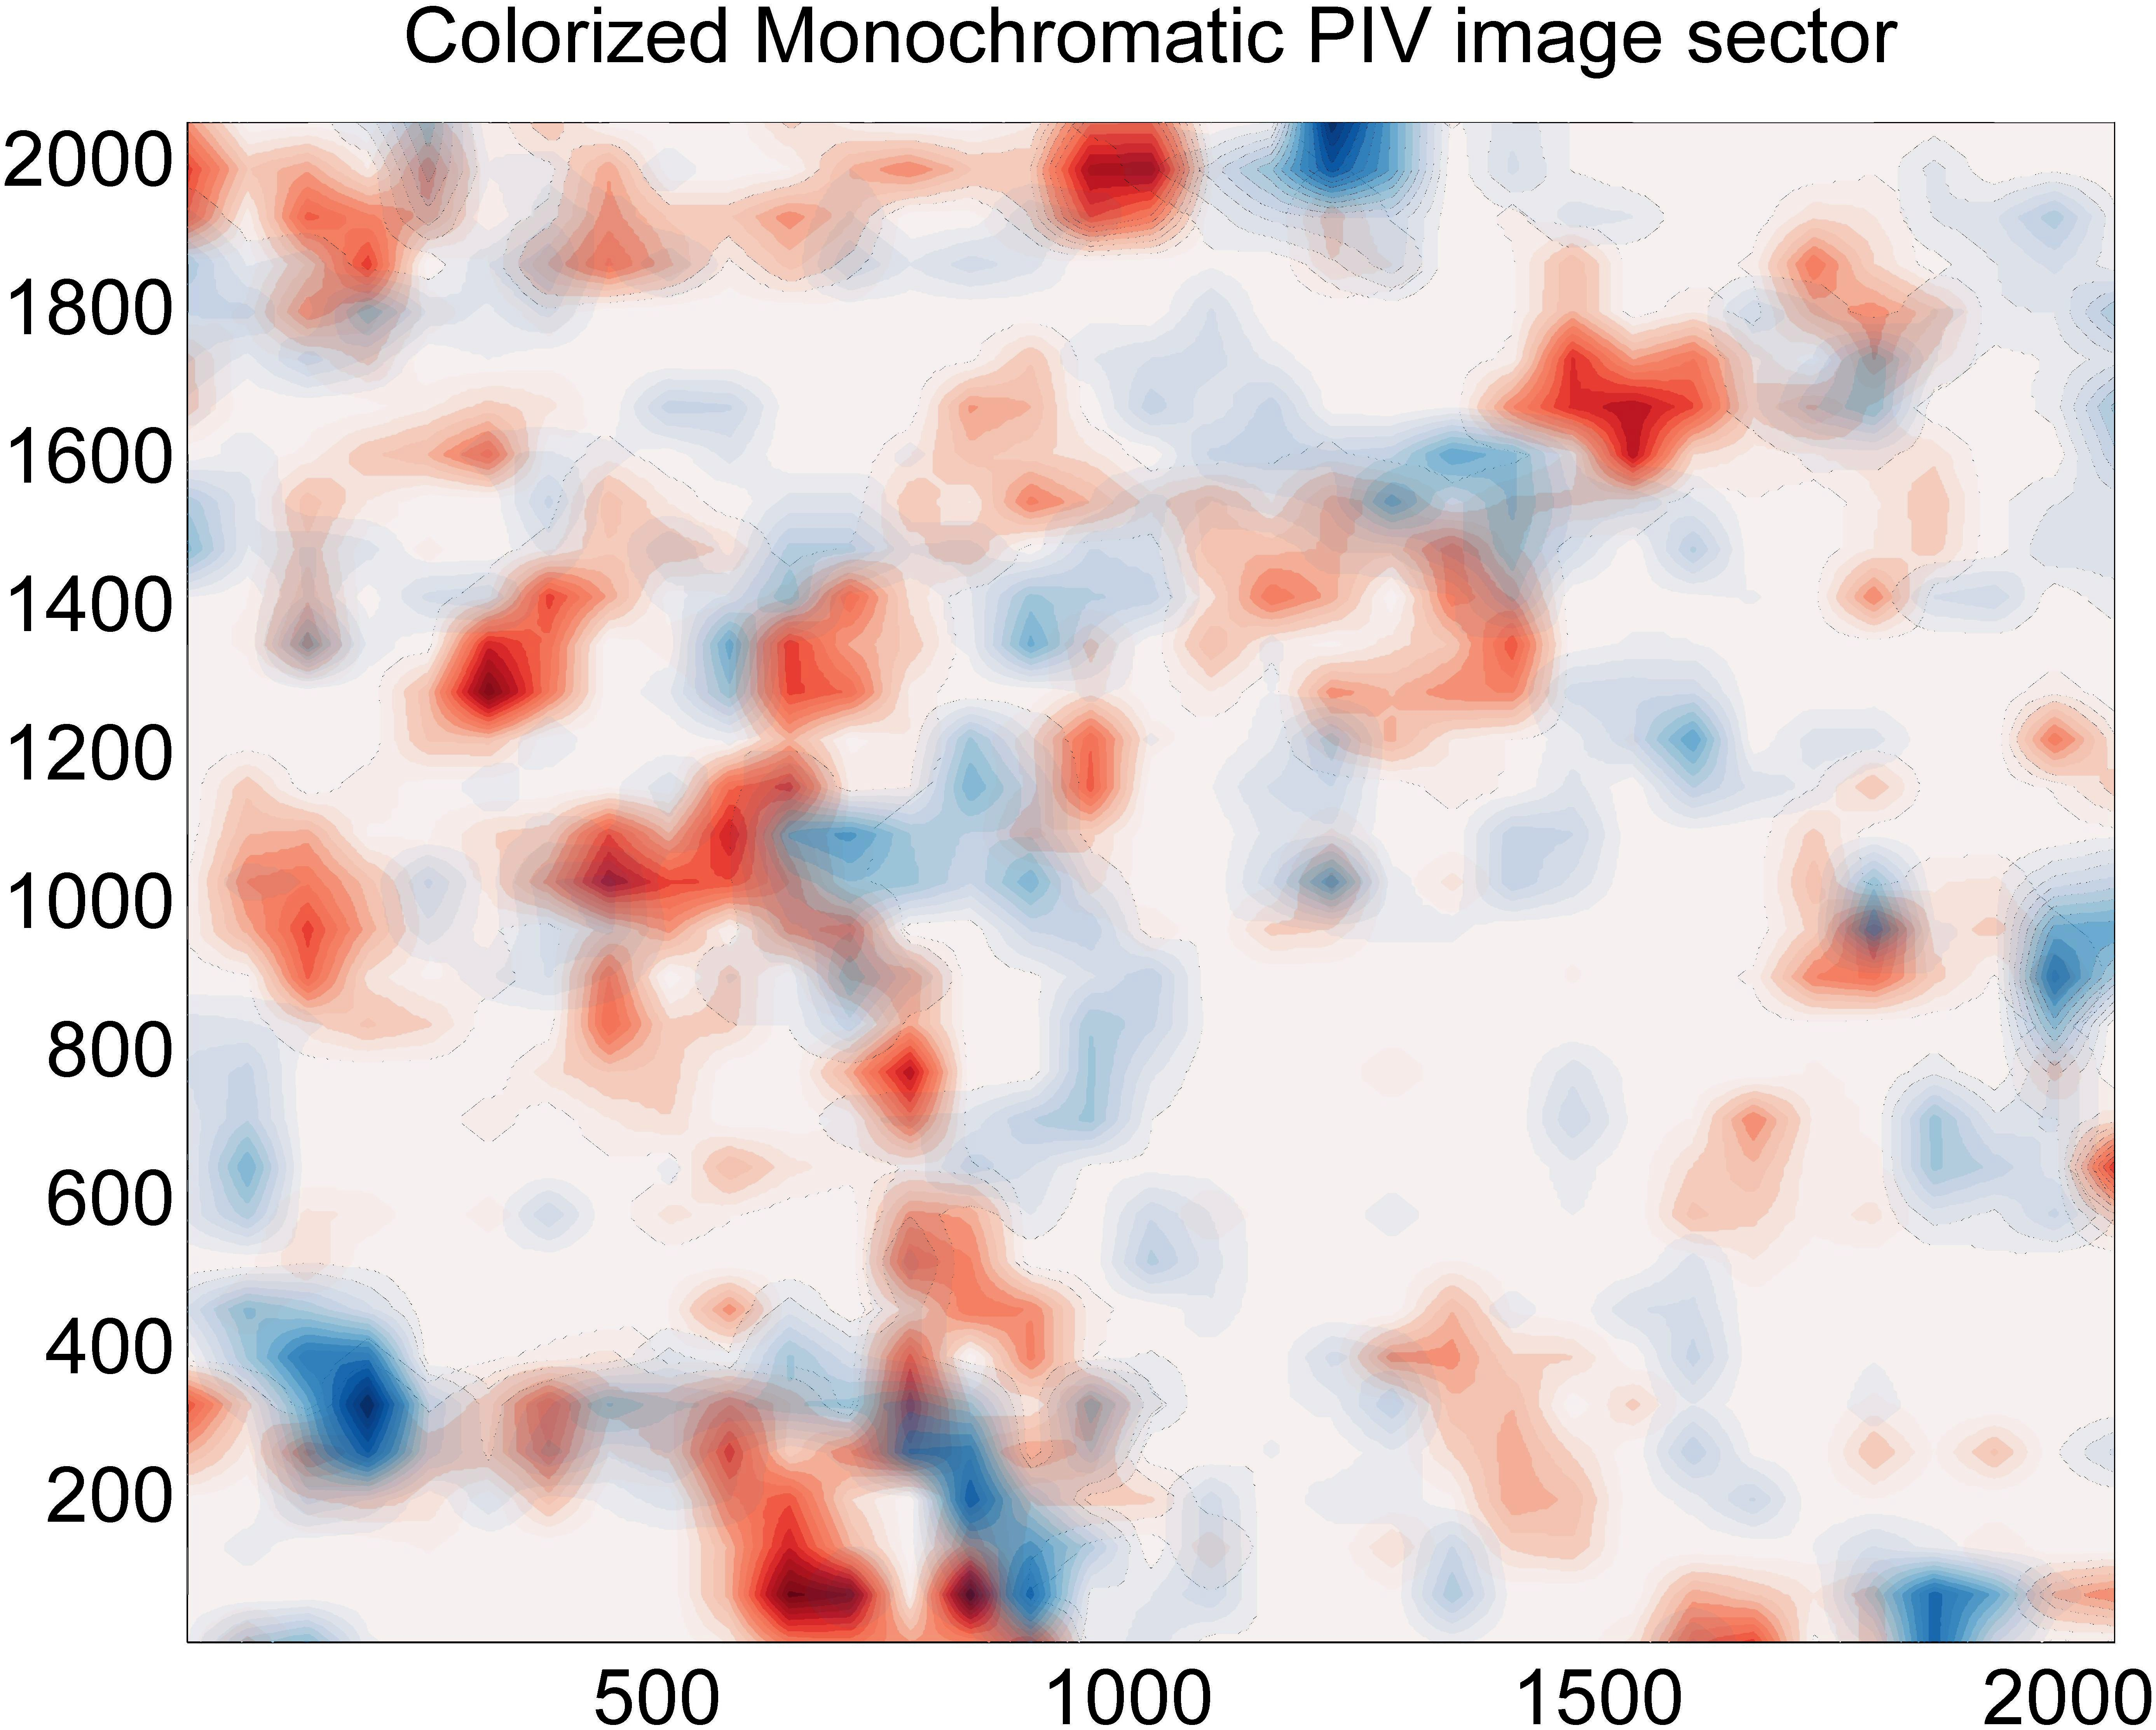
\includegraphics[width=.9\linewidth]{figs/piv_method/pive-fig_order6}
	\end{subfigure} 
	\begin{subfigure}{.49\textwidth}
		\centering
		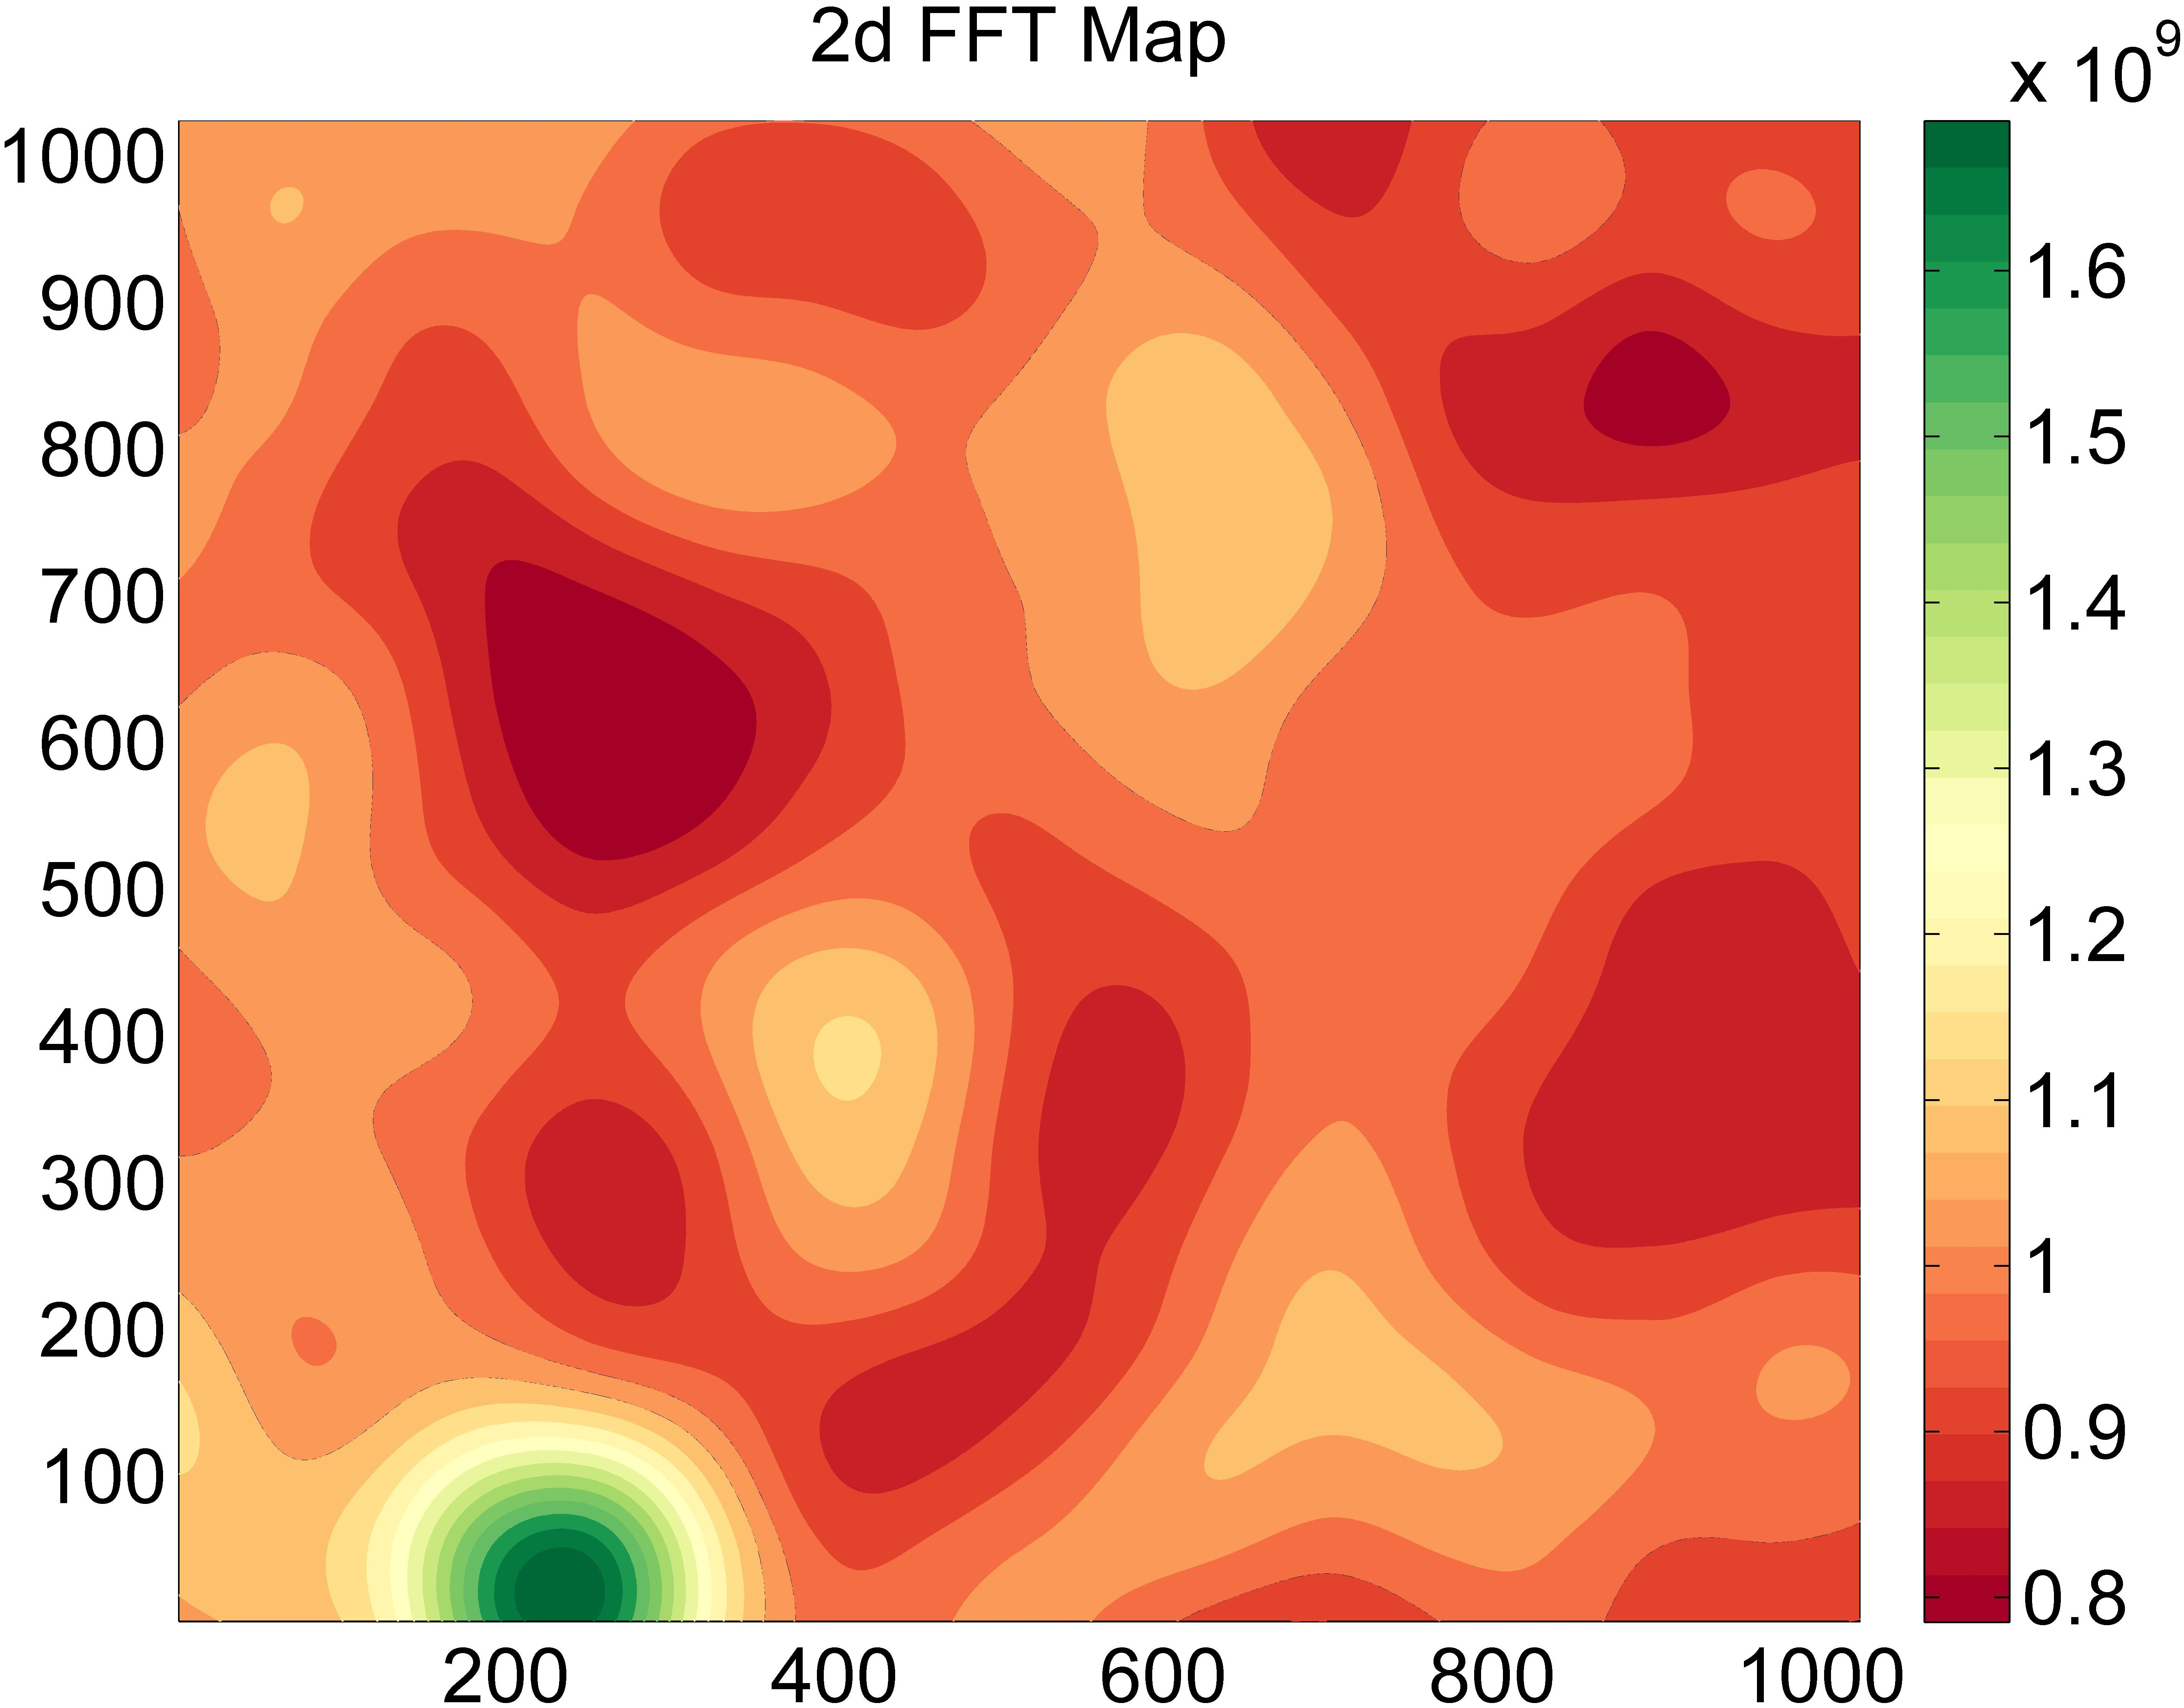
\includegraphics[width=.9\linewidth]{figs/piv_method/pive_fft_order6}
	\end{subfigure}	
	\caption{Overlaid sector snapshots (left) and corresponding correlation 
		map (right), 6th order up sampling.}
	\label{fig:piv_sector_overlay_fft_6up}
\end{figure}
\vspace{16pt}

Since the sampling method creates a finer mesh, the sub-pixel resolution 
increases. Table \ref{table:piv_upsampling_displacement} shows how the 
displacement error may vary with sampling order.

\begin{table}[H]
\begin{center}
\begin{tabular}{|ccc|}
	\hline
	Order & $x_{disp}$ & $y_{disp}$\\
	\hline
	0 & 4 & 0\\
	1 & 3.5 & 0.5\\
	2 & 3.75 & 0.25\\
	3 & 3.625 & 0.25\\
	4 & 3.625 & 0.3125\\
	5 & 3.625 & 0.3125\\
	6 & 3.6406 & 0.2969\\
	7 & 3.6406 & 0.2969\\
	\hline
\end{tabular}
\caption{Pixel displacements by up sampling order.}
\label{table:piv_upsampling_displacement}
\end{center}
\end{table}


While the above analysis demonstrates the mathematical motivation behind up 
sampling images before performing the Fourier transform for measuring particle 
displacement, it does not adequately describe the total uncertainty in 
measurements made with particle image velocimetry. The uncertainty associated 
with measurements made with PIV are dependent upon the geometry of the specific 
optical setup used to gather the data.

In stereo PIV,  the 
derivative terms which relate displacements in the image plane to displacements 
in the real plane (Equations \ref{eq:piv_to_real1} to \ref{eq:piv_to_real4}) 
are not constant throughout the entire interrogation plane. They are instead 
functions of the pixel position. These functions can be determined by 
measurement of a calibration target, which has a pattern of dots of known 
position. The known position of these calibration points can 
be used to compute the nine coefficients for four functions of the form in 
Equation \ref{eq:calibration_equation}. There exists a separate set of nine 
coefficients for the left and right camera, in the $X$ and $Y$ directions.

\begin{equation}
	\begin{multlined}
	X_{mm} =  [A + B(X_{px}) + C(Y_{px}) + D(Z_{mm}) + E(X_{px}^2) + \\
	F(Y_{px}^2) + G(X_{px}Z_{mm}) + H(Y_{px}Z_{mm}) + J(X_{px}Y_{px})]
	\end{multlined}
	\label{eq:calibration_equation}
\end{equation}
\newline
\noindent
where $X_{mm}$ is the position in $mm$, $[A, B, C, D, E, F, G, H, J]$ 
represents the entire set of nine coefficients, $X_{px}$ and $Y_{px}$ are the 
pixel positions in the $X$ and $Y$ directions of the camera plane 
respectively. Similarly $Z_{mm}$ is the actual position in the $Z$ direction. 
The 
$Z_{mm}$ position of all particles is assumed to be zero in the first image, 
and is determined relative to its starting position by the root mean square of 
the solutions to Equations \ref{eq:piv_to_real1} through \ref{eq:piv_to_real4}.
For simple optical setups, this approach also accounts for distortion due to 
variations in magnification \cite{soloff1997, willert1997}.


